% Szkielet dla pracy inżynierskiej pisanej w języku angielskim.

\documentclass[english,bachelor,a4paper,twoside]{ppfcmthesis}

\usepackage[utf8]{inputenc}
\usepackage[OT4]{fontenc}
\usepackage[T1]{fontenc}
\usepackage{graphicx}
\usepackage{listings}
\usepackage{xcolor}
\usepackage{pifont}

\newcommand*\OK{\ding{51}}

\definecolor{codestrings}{rgb}{0.164,0,1}
\definecolor{codecomment}{rgb}{0.25,0.49,0.37}
\definecolor{codekeywords}{rgb}{0.8,0,0.33}
\definecolor{codebackground}{rgb}{0.95,0.95,0.95}
\lstdefinestyle{cblockstyle}{
	inputencoding=utf8,
	language=C++,
	extendedchars=true,
	basicstyle=\ttfamily\footnotesize,
	numbers=left,
  	numbersep=3pt,
	framexleftmargin=2pt,
  	framerule=0pt,
  	frame=lines,
	numberstyle=\tiny,
	tabsize=2,
	showstringspaces=false,
	showspaces=false,
	  keywordstyle=\bfseries\color{codekeywords},
	  identifierstyle=\color{black},
	  stringstyle=\color{codestrings},
	  commentstyle=\color{codecomment},
	  columns=fullflexible,
	  abovecaptionskip=\medskipamount,
	  belowcaptionskip=\medskipamount,
	  backgroundcolor=\color{codebackground},
}
\lstdefinestyle{pblockstyle}{
	inputencoding=utf8,
	language=python,
	extendedchars=true,
	basicstyle=\ttfamily\footnotesize ,
	numbers=left,
  	numbersep=3pt,
	framexleftmargin=2pt,
  	framerule=0pt,
  	frame=lines,
	numberstyle=\tiny,
	tabsize=2,
	showstringspaces=false,
	showspaces=false,
	  keywordstyle=\bfseries\color{codekeywords},
	  identifierstyle=\color{black},
	  stringstyle=\color{codestrings},
	  commentstyle=\color{codecomment},
	  columns=fullflexible,
	  abovecaptionskip=\medskipamount,
	  belowcaptionskip=\medskipamount,
	  backgroundcolor=\color{codebackground},
}
\lstdefinestyle{clinestyle}{
	tabsize=2,
	frame=lines,
	inputencoding=utf8,
	language=C++,
	keywordstyle=\bfseries\color{codekeywords},
	identifierstyle=\color{black},
	stringstyle=\color{codestrings},
	commentstyle=\color{codecomment},
	basicstyle=\ttfamily,
}
\lstnewenvironment{cblock}{\lstset{style=cblockstyle}}{}
\lstnewenvironment{clinee}{\lstset{style=clinestyle}}{}
\lstnewenvironment{pblock}{\lstset{style=pblockstyle}}{}
\graphicspath{ {figures/} }

% Authors here.
\author{%
   Michał Kempka \album{105256} \and 
   Grzegorz Runc \album{109759} \and 
   Jakub Toczek \album{109704} \and 
   Marek Wydmuch \album{109746}}
\authortitle{}                                        % Do not change.
\title{VIZIA: 3D Video Game-based Environment for Research on Learning Agents from Raw Visual Information}        % Note how we protect the final title phrase from breaking (~zamiast spacyj)
\ppsupervisor{~Wojciech Jaśkowski,~Ph.~D.} % Your supervisor comes here.
\ppyear{2016}                                         % Year of final submission (not graduation!)

\begin{document}
\lstset{breaklines=true,
    postbreak=\raisebox{0ex}[0ex][0ex]{\ensuremath{\color{red}\hookrightarrow\space}}}
% Front matter starts here
\frontmatter\pagestyle{empty}%
\maketitle\cleardoublepage%

% Blank info page for "karta dyplomowa"
\thispagestyle{empty}\vspace*{\fill}%
\begin{center}Tutaj przychodzi karta pracy dyplomowej;\\oryginał wstawiamy do wersji dla archiwum PP, w pozostałych kopiach wstawiamy ksero.\end{center}%
\vfill\cleardoublepage%

%Streszczenie i abstrakt
\chapter*{Streszczenie}

Niniejsza praca jest poświęcona wykorzystaniu trójwymiarowych gier typu FPS (ang. first-person shooter) do badań nad inteligentnymi agentami, które działają i uczą się w oparciu o informację obrazową.

W ciągu ostatnich lat komputery znacznie przewyższyły ludzi pod względem możliwości prze-twarzania surowych danych.
Nie dotyczy to jednak przetwarzania informacji obrazowej, w przypadku której postęp dotyczy tylko ograniczonych zastosowań.
Konwolucyjne sieci neuronowe z powodzeniem są wykorzystywane do klasyfikacji zdjęć, a w połączeniu z uczeniem ze wzmocnieniem znajdują zastosowanie m.in. w robotyce.
Głębokie uczenie ze wzmocnieniem zostało również wykorzystane do nauczenia agenta grania w 7 gier z Atari 2600.
Przestrzeń praktycznych zastosowań jest jednak w tym przypadku ograniczona, ponieważ jest to informacja obrazowa o dwuwymiarowym charakterze.
Dodanie aspektu głębi, a zatem wykorzystanie gier trójwymiarowych, znacznie zwiększyłoby możliwość praktycznych zastosowań.
Ze względu na obserwowanie świata z perspektywy pierwszej osoby szczególnie interesujące pod tym względem wydają się być gry FPS, jednak dotychczas nie prowadzono badań nad wykorzystaniem uczenia ze wzmocnieniem z informacji obrazowej pochodzącej z gry FPS.

Celem pracy było opracowanie łatwego w użyciu środowiska do badań nad inteligentnymi agentami, które działają i uczą się w oparciu o informację obrazową generowaną przez trójwymiarową grę FPS, oraz przeprowadzenie eksperymentów dla prostych scenariuszy.

Rezultatem niniejszej pracy jest środowisko VIZIA oparte na grze Doom dostosowane do potrzeb paradygmatu uczenia ze wzmocnieniem.
Stworzony został interfejs programistyczny zaimplementowany w C++ pozwalający na wykonywanie akcji, pobieranie obrazu i informacji o bohaterze gry, jak i swobodny dobór parametrów wykonania gry.
Parametry te mogą być zapisywane w postaci plików konfiguracyjnych.
Zapewniono również wsparcie dla Pythona i Javy.
Środowisko to wspiera tworzenie scenariuszy testowych w zewnętrznych edytorach i implementację funkcji nagrody za pomocą języka skryptowego Action Code Script.
Poza trybem pełnej kontroli nad grą zaimplementowano również tryb obserwatora, pozwalający na uczenie agenta na podstawie rozgrywki prowadzonej przez człowieka.
Dodatkowo środowisko może pracować w trybie zarówno synchronicznym, w którym gra czeka na akcje agenta, jak i asynchronicznym, w którym gra działa ze stałą prędkością, co pozwala na wykorzystanie jej w rozgrywkach sieciowych.

Stworzone oprogramowanie zostało przygotowane do pracy w systemie Linux i udostępnia tryb niewymagający środowiska graficznego, dzięki czemu może być uruchamiane na zdalnych stanowiskach.
Środowisko umożliwia przetwarzanie z prędkościami liczonymi w tysiącach klatek na sekundę.

Przeprowadzone dla prostych środowisk testowych eksperymenty wykorzystujące uczenie ze wzmocnieniem głębokich sieci neuronowych wskazują na użyteczność stworzonego środowiska do badań nad głębokim uczeniem ze wzmocnieniem z informacji obrazowej.
	
\chapter*{Abstract}

This thesis is concentrated on usage of 3-dimensional FPS games in research on intelligent agents that act and learn based on purely visual information.


In the last couple of years computers significantly exceeded humans in terms of raw data processing.
It does not apply, however, to visual information processing, which has been equally successful only for certain applications.
Convolutional Neural Networks are successfully used for image classification, and combined with reinforcement learning they prove to be useful in robotics, among others.
Deep reinforcement learning has also been employed to teach an intelligent agent to play 7 Atari 2600 games.
However, range of practical applications of such technology is very limited, as it works with visual input which is two-dimensional.
Adding the depth, thus involving games in three-dimensional environments, would notably increase real-life practicality.
Due to first-person perspective, First-person shooter games (FPS) are especially interesting. However, no research has been conducted so far, that involves reinforcement learning from raw visual data generated by an FPS game.

The main aim of this thesis was to create an easy-to-use environment for research on intelligent agents that act and learn based on purely visual data generated by a three-dimensional FPS game, and conducting simple experiments for the most basic scenarios.


Work on this thesis resulted in creation of environment employing a vintage game --- Doom to expose an interface proper for reinforcement learning --- VIZIA. VIZIA's application programming interface was fully written in C++ and allows making in-game actions, retrieve game's screen buffer and plenty of in-game parameters such as player's health or ammunition. 
The API offers a myriad of configuration options which can easily be written and stored in text files.
In addition to C++ support bindings for Python and Java has been created as these languages are more popular for AI research purposes. 
The environment offers a mechanism of scenarios that enables researchers to design custom research conditions that support reinforcement learning paradigm.
What is more, multiple different modes of operation are available and allow taking full control over game's engine processing, perform apprenticeship learning or even engage in multiplayer/multiagent skirmishes. 

VIZIA is mainly targeted at Linux platform and provides options for off-screen rendering that requires no graphical environment, therefore can be used with remote terminals.
The environment allows reaching processing speeds counted in thousands of frames per second.

In order to test practicality of using VIZIA in AI research, a simple experiment has been conducted that in fact proves that the environment serves its purpose.
\cleardoublepage

% Table of contents.
\pagenumbering{Roman}\pagestyle{ppfcmthesis}%
\tableofcontents* \cleardoublepage%

% Main content of your thesis starts here.
\mainmatter%



\chapter{Introduction}
\label{ch:introduction}
\section{Motivation}
\label{sec:motivation}

Visual signals are one of the main sources of information about the surrounding environment for humans and animals.
While computers have already greatly exceeded humans in terms of raw data processing, they still do not match their ability to process images.
However, recent increase in computing power and emergence of affordable technologies allowing to perform general computations on graphics cards (CUDA, OpenCL) enabled significant progress in this area.
An important part of this advance are deep convolutional neural networks (CNNs).


CNNs for the first time came into prominence when they were used to classify 1.6 millions images into 1000 classes~\cite{NIPS2012_4824}.
This solution was so effective that now this is the prevalent method of image classification.
This success hugely popularized CNNs and soon enough they were used for much more complex tasks.
In combination with reinforcement learning, they were used to model intelligent agent which attempted playing 7 Atari 2600 games from Arcade Learning Platform\cite{mnih-atari-2013}.
In 6 of them the achieved results were better than in all the previous approaches, and in the case of 3 results were better than those achievable by human players.

The main drawback of Atari games is that they are only two-dimensional, so their usability at solving real-world problems is quite limited, but reinforcement learning itself was successfully used for identifying features in static images \cite{conf/cvpr/GoodrichA12} and in robotics for controlling racing slot car using only image from the camera \cite{rieijcnn12} and even for steering RC helicopter\cite{Abbeel07anapplication}.
Bigger scope of practical applications is offered by 3D games which are a better approximation of the real-world.
% <---
Among 3D games, First Person Shooter (FPS) games are particularly interesting because the first-person perspective is a good equivalent of the image obtained from the mobile robot vision systems.
Also important is their great popularity, and simple game rules make it easy to implement rewarding mechanism.
% >---

FPS games have already been successfully used in research on artificial intelligence, especially the most popular ones such as Unreal Tournament \cite{6314567} \cite{6922494}, Counter-Strike \cite{5035619} or Quake III Arena \cite{el2007hybrid}.
However, in these studies agents acted upon high-level information like positions of walls, enemies, locations of item etc, which are normally inaccessible to human player.
Supplying only raw visual information would relieve researchers of the burden of supplying AI high-level information and handcrafted features.
What is more it would force agents to become more autonomous and behave in a way more resembling real intelligent agents (humans and animals).
So far no studies have been conducted on the reinforcement learning from visual information obtained from 3D FPS games.


Currently there are no environments that allow using FPS games for research on artificial intelligence algorithms, in which agents rely exclusively on raw visual information.
This could be a serious factor that is impending the progress of visual information-based research on reinforcement learning.
Engaging in that kind of research would require a large amount of work associated with creation of an environment integrating game engine with interface suited to reinforcement learning paradigm.
The existence of such a tool would allow conducting experiments and focus on the goal of research without having to worry about availability of the test environments.
 

\section{Aims and scope}
%%W rozdziale 1 nie pojawia sie nazwa VIZIA
The main aim of this thesis is, thus Section~\ref{sec:motivation}, to create an easy to use and flexible environment for research on intelligent agents that work and learn using the raw visual information generated by the engine of 3D FPS game. 
% <---
In order to confirm usability of the created environment experiments on simple scenarios should be conducted.
% >---

The goal will be achieved by meeting the following objectives:
\begin{itemize}
 \item to compare and select needed technologies,
 \item to implement the environment,
 \item define API,
 \item to define and implement test scenarios in the created environment,
 \item to implement learning algorithms for deep neural networks,
 \item to conduct experiments for simple test scenarios.
\end{itemize}
% <---
It was assumed that VIZIA environment has to meet the following assumptions:


\begin{enumerate}
\item based on popular open-source 3D FPS game (ability to modify the code and the freedom of publication)
\item lightweight (portability and the ability to run multiple instances)
\item fast (AI should be a limiting factor for the speed of processing, not the game itself)
\item total control over game's processing (pausing processing for the duration of AI run)
\item customizable resolution and rendering parameters (adjusting the image generated by the game to meet the needs)
\item multiplayer (testing agent in the fight against the human player or other AI)
\item spectator mode (agent learning from observations of a human playing)
\item easy and convenient creation of custom scenarios (creating test environments tailored to the needs)
\item reinforcement learning friendly API in C++ (use for the research on reinforcement learning; the ability to bind other languages)
\item Python bindings (popularity of Python in machine learning)
\item multiplatform (availability of full functionality on Linux, Windows and Mac OS)
\end{enumerate}

% >---
	
\section{Thesis organization}


This thesis is structured as follows. 
Chapter~\ref{ch:architecture} gives an overview of technologies and tools used to develop the VIZIA environment and describes environment's architecture. It addresses design decisions and problems and contains result of performance tests. 
Chapter~\ref{ch:api} presents the designed application programming interface, python binding and shows API's usage examples. 
Chapter~\ref{ch:scenarios} gives definition of scenario and presents tools and methods for creating scenarios. It contains the description of designed scenarios. 
Chapter~\ref{ch:experiment} shows methods used for conducting experiments and their results. 
Chapter~\ref{ch:conclusions} concludes this thesis and proposes directions for future work.

\section{Contributions}
	\subsection{Engineering Project}
	\begin{description}
		\item[Michał Kempka] \hfill
			\begin{itemize}
				\item part of interface design,
				\item testing and experiments,
				\item part of Python binding,
				\item Python examples,
				\item scenarios creation,
				\item support for configuration files.
			\end{itemize}
		\item[Grzegorz Runc] \hfill
			\begin{itemize}
				\item generation of depth buffer,
				\item support for off-screen rendering.
			\end{itemize}
		\item[Jakub Toczek] \hfill
			\begin{itemize}
				\item Python binding,
				\item Java binding.
			\end{itemize}
		\item[Marek Wydmuch] \hfill
			\begin{itemize}
				\item VIZIA API design,
				\item VIZIA API implementation,
				\item VIZIA module in Doom engine implementation,
				\item CMake configuration.
			\end{itemize}
	\end{description}
	
   	
	\subsection{Thesis}
	\begin{description}
		\item[Michał Kempka] \hfill
			\begin{itemize}
				\item foundations for Chapter \ref{ch:api},
				\item Chapter \ref{ch:scenarios},
				\item Chapter \ref{ch:experiment},
				\item Chapter \ref{ch:conclusions},
				\item translation of the abstract.
			\end{itemize}
		\item[Grzegorz Runc] \hfill
			\begin{itemize}
				\item Chapter~\ref{ch:introduction},
				\item Section~\ref{sec:technologies}.
                \item the abstract
			\end{itemize}
		\item[Jakub Toczek] \hfill
			\begin{itemize}
				\item Chapter~\ref{ch:api}.
			\end{itemize}
		\item[Marek Wydmuch] \hfill
			\begin{itemize}
				\item Section~\ref{sec:architecture},
				\item Section~\ref{sec:architecture_solutions},
				\item Section~\ref{sec:performance},
			\end{itemize}
	\end{description}

\chapter{Framework Architecture}
\label{ch:architecture}
\section{Used Technologies}
\label{sec:technologies}

\subsection{3D FPS Game Engine}

%TA SEKCJA MNIE DEMOTYWUJE
%MNIEJ BOLAŁO PISANIE MOTYWACJI
%MIMO CZASU JAKI TRZEBA BYŁO NA NIĄ POŚWIĘCIĆ

%Nad ta sekcja warto jeszcze popracowac. Troche wiecej daloby sie tutaj napisac, np. jak zostalo ocenione code complexity i brand recognition. W wielu miejscach brakuje tutaj logicznego przeplywu mysli i sekcja jest dosc chaotyczna.

\begin{figure}
\centering
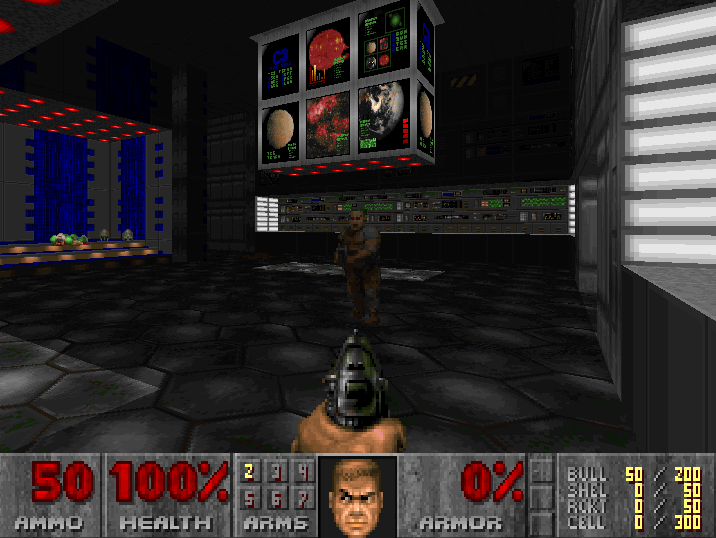
\includegraphics[scale=0.5]{doom.png}
\caption{Screenshot of Doom}
\label{fig:doom}
\end{figure}

VIZIA Environment was build around FPS game Doom. 
The environment uses  modernized version of Doom's Boriginal engine --- ZDoom~\cite{zdoom-main}. 
Screenshot from the game is shown in Figure~\ref{fig:doom}.
Doom was chosen out of 6 other recognizable FPS games considered: 

\begin{itemize}
\item Quake III Arena 
\item Doom 3
\item Half-Life 2 
\item Unreal Tournament 2004
\item Unreal Tournament
\item Cube
\end{itemize}
The comparison between them is shown in Table~\ref{tab:engines}.
% <--
Some of the criteria had to be subjective (System requirements, Code complexity), because they were based on analysis of game engine's code in the context of internal architecture, easiness of modification and performance. 
As brand recognition was treated a number (in millions) of Google results of 20.10.2016 for phrases containing only the brand name e.g., `doom' for Doom and Doom 3, `unreal tournament' for Unreal Tournament 2004 and Unreal Tournament etc.
Game was considered as able to generate small resolution image if it is possible to set resolution to smaller than 640x480.
Selecting the game was done by discarding those not meeting requirements deemed necessary.
% >--

\begin{table}[]
\centering
\caption{Overview of 3D FPS games considered as base of VIZIA Environment}
\label{tab:engines}
\begin{tabular}{|p{2cm}||p{1.3cm}|p{1.3cm}|p{1.3cm}|p{1.3cm}|p{1.3cm}|p{1.3cm}|p{1.3cm}|}
\hline
Game                      & Quake III: Arena \cite{quake1}~\cite{quake2} & Doom \cite{doomreq}~\cite{zdoom}~\cite{zdoom-wiki}  & Doom 3 \cite{d3req}~\cite{idtech4}    & Half-Life 2 \cite{half2}~\cite{source} & Unreal Tournament 2004 \cite{ut04rqe}~\cite{ue2} & Unreal Tournament \cite{ue4req}~\cite{ue4faq} & Cube~\cite{cube}        \\ \hline
Game Engine               & ioquake3         & zdoom & id tech 4 & Source      & Unreal Engine 2        & Unreal Engine 4   & Cube Engine \\ \hline
Release year               & 1999             & 1993  & 2003      & 2004        & 2004                   & --\footnotemark              & 2001        \\ \hline
Open Source               & \OK              & \OK   & \OK       &             &                        & \OK               & \OK         \\ \hline
License                   & GPLv2            & GPL   & GPLv3     & Closed      & Closed                 & Custom            & ZLIB        \\ \hline
Language                  & C                & C++   & C++       & C++         & C++                    & C++               & C++         \\ \hline
DirectX                   &                  &       & \OK       & \OK         &                        & \OK               &             \\ \hline
OpenGL                    & \OK              & \OK\footnotemark   & \OK       & \OK         & \OK                    & \OK               & \OK         \\ \hline
Software Render           &                  & \OK   &           &             &                        &                   &             \\ \hline
Windows                   & \OK              & \OK   & \OK       & \OK         & \OK                    & \OK               & \OK         \\ \hline
Linux                     & \OK              & \OK   & \OK       & \OK         & \OK                    & \OK               & \OK         \\ \hline
Mac OS                    & \OK              & \OK   & \OK       & \OK         & \OK                    & \OK               &             \\ \hline
Scripting                 &                  & \OK   & \OK       & \OK         & \OK                    & \OK               & \OK         \\ \hline
Custom assets             & \OK              & \OK   & \OK       & \OK         & \OK                    & \OK               & \OK         \\ \hline
Map editor                & \OK              & \OK   & \OK       & \OK         & \OK                    & \OK               & \OK         \\ \hline
Multiplayer               & \OK              & \OK   & \OK       &             & \OK                    & \OK               & \OK         \\ \hline
Engine access             & Code             & Code  & Code      & SDK         & SDK                    & Code               & Code        \\ \hline
Small resolutions         & \OK              & \OK   & \OK       & \OK         & \OK                    & \OK               & \OK         \\ \hline
Screen buffor access      & \OK              & \OK   & \OK       &             &                        & \OK               & \OK         \\ \hline
System requirements       & Low              & Low   & Medium    & Medium      & Medium                 & High              & Low         \\ \hline
Disk space                & 70MB             & 40MB  & 2GB       & 4,5GB       & 6GB                    & \textgreater10GB\footnotemark  & 35MB        \\ \hline
Code complexity           & Medium           & Medium& High      & NA          & NA                     & High              & Low         \\ \hline
Brand recognition         & 41,1             & 99    & 99        & 36,6        & 1,2                    & 1,2               & 0,1         \\ \hline
Active community          & \OK              & \OK   & \OK       & \OK         &                        & \OK               &             \\ \hline
Free original assets      &                  &       &           &             &                        & \OK               & \OK         \\ \hline
\end{tabular}
\end{table}
\addtocounter{footnote}{-2}
\footnotetext{Unreal Tournament is in pre-alpha phase; release date is unknown.}
\stepcounter{footnote}
\footnotetext{GZDoom, ZDoom fork, is OpenGL based.}
\stepcounter{footnote}
\footnotetext{Disk requirements are yet unknown, but they will be greater than requirements of Unreal Engine 4.}
  
% <-- MOCNO ZMODYFIKOWANE, WRĘCZ NA NOWO NAPISANE
Unreal Tournament 2004 had to rejected because its engine is only accessible by Software Development Kit~(SDK) and it lacks support for controlling speed of execution and direct screen buffer access.
The game was not prepared to be heavily modified and its use in research was so far limited to server modifications.

Similar problems would have to be overcome in case of Half-Life 2, although Source engine is widely known for modding capabilities.
Although the lack of multiplayer could be solved by the use of the game Counter Strike:Source or even Half-Life 2:Deathmatch, as Source engine itself has multiplayer support, it would introduce problems associated with the separation of game logic into client and server.

Client-server architecture was also the reason for the rejection of Quake III: Arena.
Despite wide recognition and active community, even access to the screen buffer and the possibility to modify the code could not overcome the lack of support for scripting.

Lack of scripting does not concern Doom 3, but its disk reqiurements was considered as a major drawback.
It had to be ignored also because of its complexity, Windows-only tools and OS-dependent rendering mechanisms.
Although its source code has been relased, it does not have united community, so there are several rarely updated versions of its sources.

Community activity is also a problem in case of Cube, as its last update was in August 2005~\cite{cube}.
However low complexity and highly intuitive map editor would make it a good choice, but its recognizably is so low that it had to be taken out of consideration. 

In case of Unreal Tournament there are no problems with recognition or lack of capabilities.
Despite active community and access to source code it was out of question, because of its very high system requirements.

% >--




Doom met most of the given requirements and allowed to implement features that would be barely achievable in other games e.g., off-screen rendering and reward computation.
The game is highly recognizable and offers support for all needed platforms.
It was also designed to work in 320x240 resolution and despite the fact that modern implementations allow bigger resolutions, it still utilizes same low resolution textures and a rendering algorithm which makes it perfect for generating small (320x240 or smaller) visual input data for AI algorithms.
In addition, its source code analysis showed that access to game logic should be easy, as its code is not object-oriented.

Unique Doom's feature is software renderer. Because of that it could be used without desktop environment (e.g., remotely over ssh) and accessing screen buffer would not require transferring it from graphics card.


\subsection{Operating System}

% <--
Development was focused on providing full functionality for Linux, while maintaining full compatibility of code with Windows and OSX. 
However, on systems other than Linux VIZIA Environment has not been thoroughly tested and build system does not support them fully.
% >--

\subsection{Game Controller and API}


The basic module for control over Doom --- game controller --- was written in C++ with usage of Boost library.
It allowed to use Boost.Interprocess library in both ZDoom and game controller, as ZDoom was written in C++.
% <--
It also made connecting game controller and game easier than it would be using low level language on the engine side and high level language for the controller.
% >--
Experimental Boost.Process library was used for control over Doom process.


Above the controller, a higher layer of abstraction was implemented defining Application Programming Interface for intelligent agents modules.
API was also developed in C++, which allowed to provide bindings to Python and Java, with possibility to add another languages e.g., Lua, Julia.


Python API was considered as the main way of controlling VIZIA Environment by users.
Bindings were prepared by using Boost.Python library.
This language is one of the most popular in data science~\cite{ds_lang} and widely known as it is taught at many universities all around the world~\cite{pythons_schools}.
There are many machine learning libraries for Python such as scikit-learn~\cite{scikit} or PyBrain~\cite{pybrain}.
Because of that, providing fully functional Python API was one of the biggest priorities of this project.


For Java bindings Java Native Interface (JNI) was used.


\subsection{Map Editor and Scripting}

Creation of game scenarios has been made possible by using tools developed by Doom community for maps and scripts editing: SLADE 3~\cite{slade3} and Doom Builder 2~\cite{db2}. Those tools utilizes ACC --- a compiler for Action Code Script (ACS), language, which is supported in ZDoom engine.
This topic was discussed further in Chapter~\ref{ch:scenarios}.

\section{Architecture}\label{sec:architecture}
	\begin{figure}
			\centering
			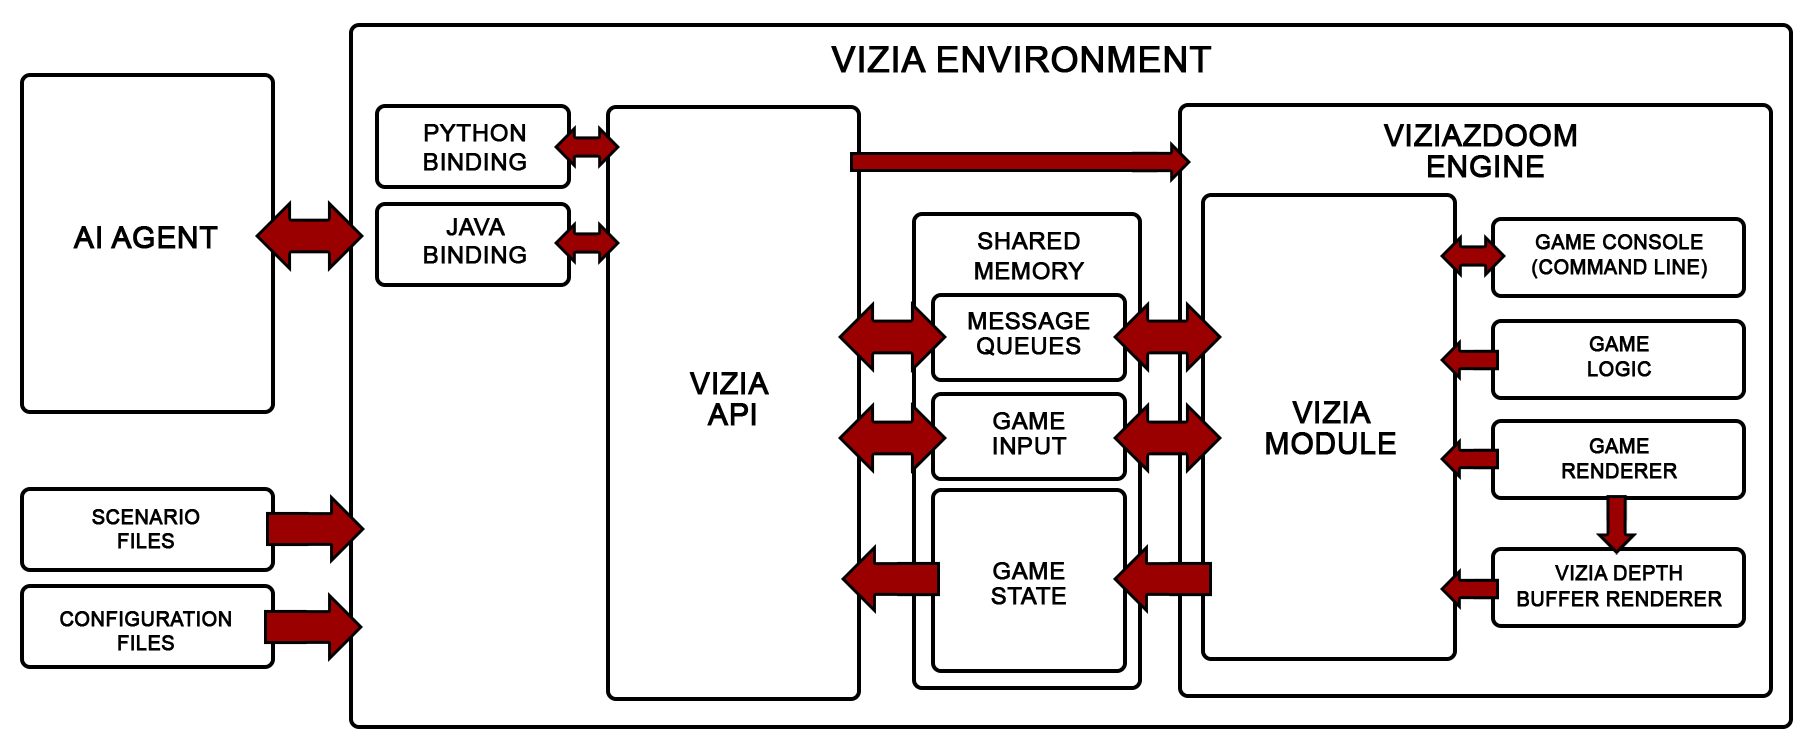
\includegraphics[scale=0.24]{architecture_diagram.png}
			\caption{Architecture of VIZIA Environment.}\label{fig:architecture_diagram}
	\end{figure}

The main components of VIZIA Environment:
    \begin{itemize}
    \item VIZIA library --- which provides a DoomGame API that allows user to configure, launch and play the game in several control modes.
    \item VIZIAZDoom --- modified ZDoom engine with a VIZIA module to communicate with a DoomGame object, control the game flow and adding additional rendering modes. It can act as a process under the control of the DoomGame object, Dome engine used for testing in Doom editors or as standalone process.
    \item Python and Java bindings --- allowing the use of the DoomGame API in these languages.
    \end{itemize}


\subsection{The separate API and game processes}\label{sec:architecture_separate_processes}

When the API user initiates the processing, the DoomGame object creates a second thread that starts VIZIAZDoom process with the appropriate settings and supervises it. From this point the API and the game communicate using only a shared memory.


\subsection{Shared memory to communicate}\label{sec:architecture_shared_memory}

During initialization set of spaces is created in the shared memory, which includes:
    \begin{itemize}
    \item A pair of message queues to control the processing flow and sending commands to the game.
    \item A shared memory area to exchange information about game input status. Both the API process and the game process reads and writes to shared memory.
    \item Shared memory areas where the game provides state of the game. These are the values of the variables necessary to control the game's processing, values of the variables available for AI agent and a copy of the game's screen. The game process saves to the memory, the process of API support.
    \end{itemize}
All shared memory spaces have unique names for each DoomGame object, which allows the coexistence of multiple instances on one machine.


\subsection{VIZIA module inside VIZIAZDoom}\label{sec:architecture_inside_viziazdoom}

VIZIA module inside the engine initializes the shared memory to exchange information with this instance of the game. Then controls the flow of the game depending on the processing mode, and received messages and determines the following processing steps:

    \begin{itemize}
    \item Starting processing of the next game tic.
    \item Transmitting commands from the message queue to the game console.
    \item Sending input information from shared memory to the game console.
    \item Processing of events that the game window received since the last tic.
    \item Rendering the current frame.
    \item Updating the information about the current game state in the shared memory.
    \end{itemize}

\subsection{Control modes}\label{sec:architecture_modes}

The DoomGame API implements four control modes:
    
    \begin{itemize}
    \item Synchronous player
    \item Synchronous spectator
    \item Asynchronous player
    \item Asynchronous spectator
    \end{itemize}
    
    \subsubsection{Synchronous player mode}\label{sec:architecture_player_mode}
    
        \begin{figure}
			    \centering
			    
\includegraphics[scale=0.24]{player_mode_diagram.png}
			    \caption{Processing flow in synchronous player mode.}\label{fig:player_mode_diagram}
	    \end{figure}
        
	    Synchronous player mode provides synchronous communication between the process that uses the API and the game process. It allows AI agent to make actions as a player. 
	    
	    In this mode, the API and the game processes communicates every tic and are waiting for each other. The game process waits until the API sends a message requesting processing of the next tic and optional update. The game process, after receiving the message, sends input information (AI agent's action) to the game console, process next game tic, and if update was requested renders the current frame and updates the information about the current game state in the shared memory. After this, the game process sends a message about completing request and starts waiting for the message processing of the next tic. The process that uses the API waits for the message about completing request.
	    
	    This mode is designed for the singleplayer mode, multiplayer mode is not supported. For more details see Section~\ref{sec::architecture_solutions}.

    \subsubsection{Synchronous spectator mode}\label{sec:architecture_spectator_mode}

	    \begin{figure}
			    \centering
			    
\includegraphics[scale=0.24]{spectator_mode_diagram.png}
			    \caption{Processing flow in synchronous spectator mode.}\label{fig:spectator_mode_diagram}
	    \end{figure}
	    
	    Synchronous spectator mode provides synchronous communication and allows AI agent to observe a human player's actions. 
	    
	    In this mode, the processes communicates every tic and are waiting for each other. The game process waits until the API sends a message requesting processing of the next tic and optional update. The game process, after receiving the message, process the window input events that have taken place since the two last update requests (last human player's action), updates the input information in the shared memory, process next game tic and if update was requested renders the current frame and updates the information about the current game state in the shared memory. After this, the game process sends a message about completing request and starts waiting for the message processing of the next tic. The process that uses the API waits for the message about completing request.

        Before processing of the next game tic the delay may be introduced in order to ensure the maximum processing speed of 35 tics per second (designed Doom ticrate).
        
        Similar to the synchronous player mode, this mode does not support multiplayer mode.

    \subsubsection{Asynchronous player mode}\label{sec:architecture_async_player_mode}

	    \begin{figure}
			    \centering
			    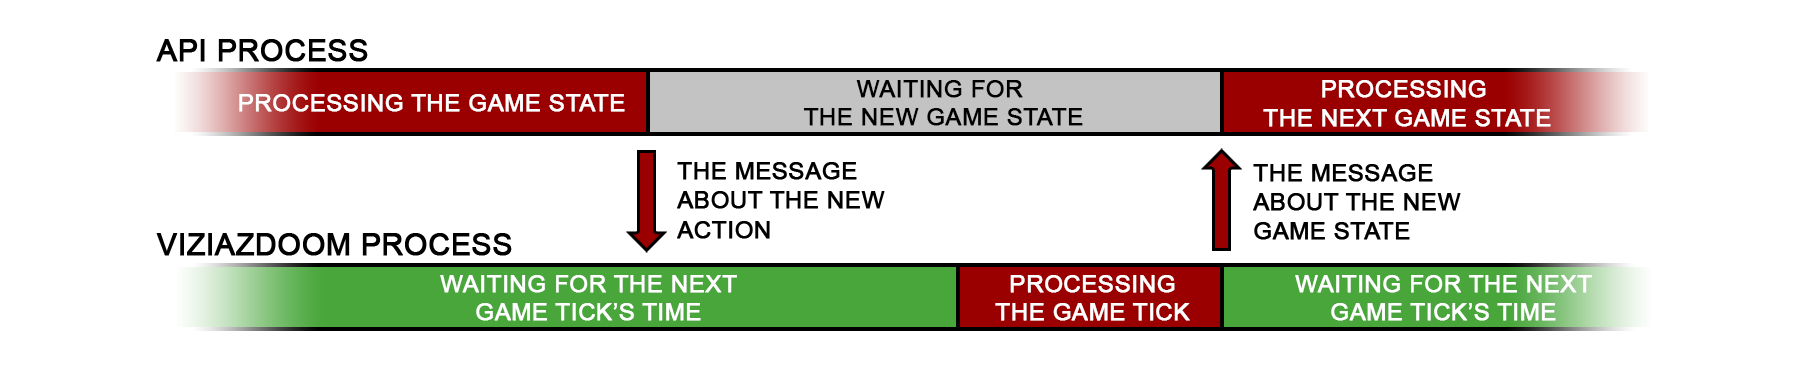
\includegraphics[scale=0.24]{async_player_mode_diagram.png}
			    \caption{Processing flow in asynchronous player mode.}\label{fig:async_player_mode_diagram}
	    \end{figure}
	    
	    Asynchronous player mode provides asynchronous communication between the process and allows AI agent to make actions as a player. 
	    
	    In this mode, the game process continuously process the game tics at a constant speed of 35 tics per second (delay is introduced between tics) without waiting for the API process. The API can send a message requesting update. Before each tic the game process checks if it received a message requesting update. After receiving such the message, it sends the input information (AI agent's action) to the game console, process next game tic, updates the information about the current game state in the shared memory, sends a message about completing request and continues processing of the game tics. The process that uses the API waits for the message about completing request.
	    
	    This mode supports both the singleplayer mode and the multiplayer mode.

    \subsubsection{Asynchronous spectator mode}\label{sec:architecture_async_spectator_mode}

	    \begin{figure}
			    \centering
			    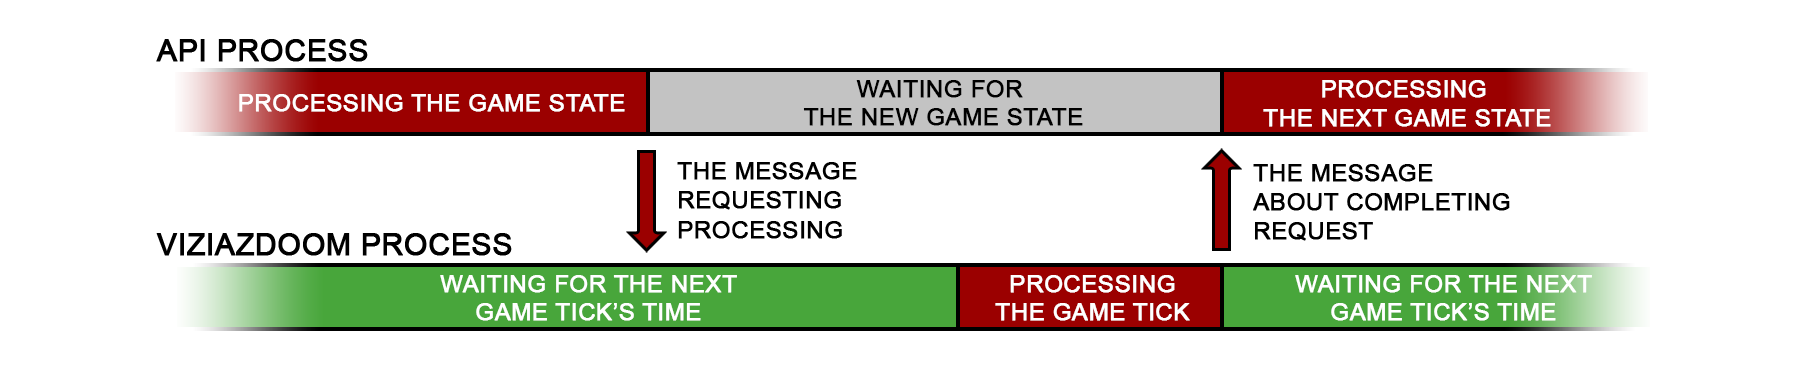
\includegraphics[scale=0.24]{async_spectator_mode_diagram.png}
			    \caption{Proce      ssing flow in asynchronous spectator mode.}\label{fig:async_spectator_mode_diagram}
	    \end{figure}
	    
	    Asynchronous spectator mode provides asynchronous communication and allows AI agent to observe a human player's actions. 
	    
	    In this mode, the game process continuously process the game tics at a constant speed of 35 tics per second without waiting for the API process. The API can send a message requesting update. Before each tic the game process checks if it received a message. After receiving such the message, it updates the input information in the shared memory (last human player's action), process next game tic, updates the information about the current game state in the shared memory, sends a message about completing request and continues processing of the game tics. The process that uses the API waits for the message about completing request.

        In this mode processing of the window input events and rendering is performed in each tic.
        
        This mode also supports both the singleplayer mode and the multiplayer mode.

\section{Other Design Decisions, Encountered problems and their Solutions}\label{sec:architecture_solutions}

\subsubsection{Why is there the separate Doom executable?}

Doom engine was designed as standalone executable. It has a different entry point for every operating system and a lot of exit points what makes it difficult to pack it inside library without making any fundamental changes to its code. In addition, this approach would not give any significant benefits. Also, leaving the Doom engine as a separate executable allows using it with Doom editors and as standalone Doom engine, which can be used for testing scenarios or human versus AI agent game in multiplayer mode.

\subsubsection{Why is shared memory used to communication?}

Shared memory is the fastest way to transfer large amounts of data between processes. It allows using the data without additional copying in the process that receives it. 
Since the game process uses shared memory only on the API request and the API process is waiting for completion of this request, additional access control mechanism (such as mutexes) is not needed.

\subsubsection{Why has depth buffer been added?}

The rendering algorithm used in ZDoom engine uses binary space partitioning (BSP) trees and other rendering techniques which does not make use of depth buffer and therefore it is not generated.
% <--
Depth buffer could be find useful for learning depth perception by agent.
In addition, information about the depth can be used to simulate the distance sensors widely used in mobile robots.  
Because of that, depth buffer was added to the engine as presented in Figure~\ref{fig:zbuffer}.
% >--
It is drawn only when demanded rendering mode includes it (see~\ref{subsec:screenformat}).
Depth is approximated by texture's scaling factor and stored as 8-bit value which gives enough accuracy and allows using it as additional color channel rather than as separate image.

\begin{figure}
\centering
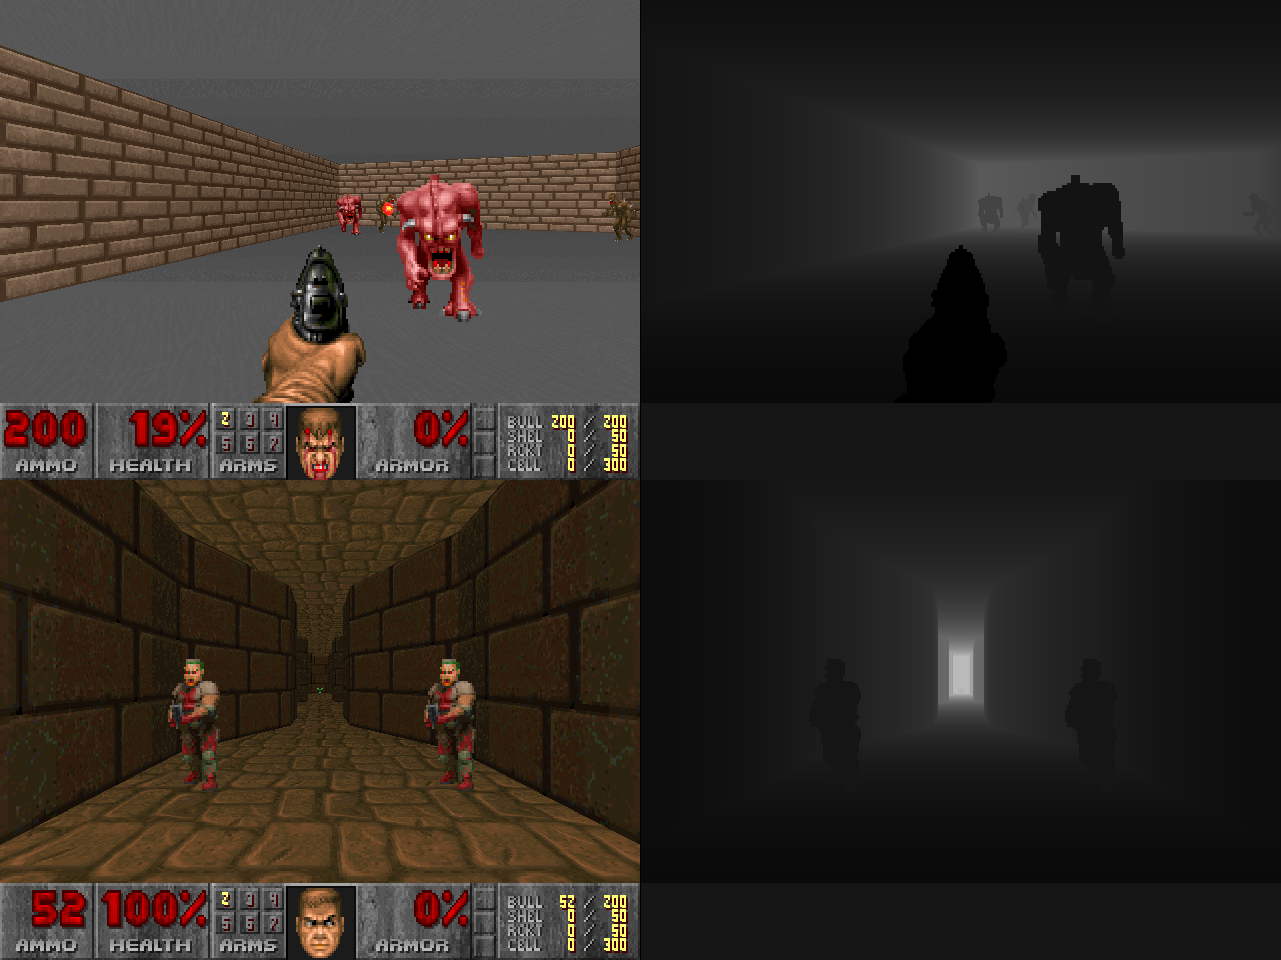
\includegraphics[scale=0.3]{zbuffer.png}
\caption{Example of implemented depth buffer}
\label{fig:zbuffer}
\end{figure}

\subsubsection{Why is multiplayer not supported in synchronous modes?}\label{sec:architecture_solution_multi}

Doom engine uses a peer-to-peer communication in multiplayer and requires synchronization between all game clients. In each tic (every 1/35th of a second) a information about input is generated and game clients should exchange it with each other. 
In synchronous modes time when next tic will be processed is unknown and may vary in different clients --- too slow or too fast processing leads to unpredictable game behaviors and errors that interrupt processing. Due to lack of time the network code has not been adapted for synchronous modes, instead it has been disabled.

\subsubsection{Why are the game and the scenario files separated?}

Doom engine uses different type of files for storing data and resources. (WAD and PK3 files) It allows loading main game resources from one file and many additional (scenario) resources from separate files. For more detailed information consult ZDoom Wiki Webpage\cite{zdoom-wiki}.

\section{Performance tests}\label{sec:performance}

All the Doom's processing including rendering is performed on a single processor thread. Additionally, rendering takes up most of the processing time. Therefore, the main factors affecting the processing speed is a geometry of the map, number of the actors (in-game objects like items and enemies) and the resolution. 

These factors have been taken into account during performance tests. Tests have been made in the synchronous player mode, where are no additional delays between tics and the image has been rendered in each tic.

	\subsection{Operating System and Hardware}
	
	Tests have been performed on the following specification:
	
	\begin{description}
		\item[Operating System] Linux Mint 17 x86\_64, kernel 3.13.0-24-generic
		\item[CPU] Intel Core i7-4790, 4x4GHz
	\end{description}

\subsection{Tests results}

\begin{figure}
\centering
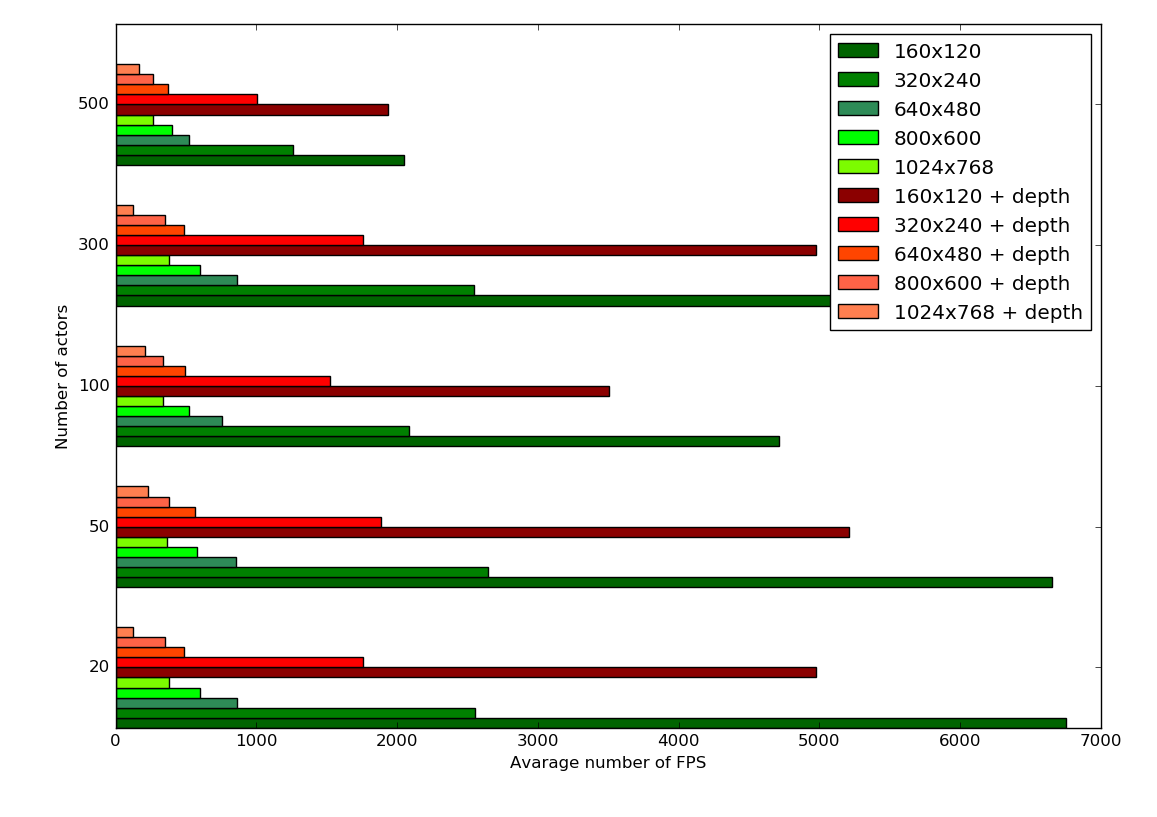
\includegraphics[scale=0.5]{result_fps.png}
\caption{Results of performance test.}
\label{fig:fps_test}
\end{figure}

Tests presented in Figure~\ref{fig:fps_test} show that the most important factor affecting performance is the rendering resolution. In case of using small resolutions, time needed to render one frame is insignificant compared to the time any reasonably good AI needs for a learning process.



\chapter{Application Programming Interface}\label{ch:api}
\section{DoomGame Methods}\label{sec:methods}
	This section documents all methods implemented by DoomGame class which is a part of Vizia namespace (C++), vizia module (Python), or vizia package (Java). DoomGame object incorporates a single instance of Doom game engine and is the way to interface with it.
	\subsection{Configuration Methods}\label{subsec:config_methods}
	Methods described in this section allows to set main parameters of the environment, such as resolution of generated image or available actions. They should be invoked after creation and before the initialization method (\emph{init}). Calling them after initialization will result in a warning or an exception, depending on severity of consequences. 
	\vspace{20pt}

\begin{clinee}
DoomGame::DoomGame();
\end{clinee}

	Constructs an instance of DoomGame. ZDoom engine is not ready for using after creation and needs initialization (init method). Freshly created DoomGame is initialized with the following parameters:
	\begin{itemize}
		\item screenResolution: RES\_320x240
		\item screenFormat: CRCGCB
		\item Game path: `./viziazdoom'
		\item Game iwad path: `./doom2.wad'
		\item map: `map01' (first map created in the iwad file if it's not changed purposefully)
		\item mode: PLAYER
		\item gameVariables: none
		\item customGameArgs: none
		\item available buttons: none
		\item rendering: all without crosshair
		\item windowVisible: \emph{true} 
		\item doomSkill: 3
		\item livingReward/deathPenalty: 0
		\item consoleEnabled: \emph{false}
		\item startEpisodeTime: 1
		\item episodeTimeout: 0
	\end{itemize}

\vspace{20pt}
\begin{clinee}
DoomGame::~DoomGame();
\end{clinee}
	Destroys DoomGame object and safely ends work of the environment.


\vspace{20pt}
\begin{clinee}
bool DoomGame::init();
\end{clinee}

	Initializes the environment and spawns the Doom engine process. Configuration cannot be changed after calling \emph{init} method. Init returns \emph{true} when the game engine was started properly and \emph{false} otherwise. 


\vspace{20pt}
\begin{clinee}
bool DoomGame::loadConfig(std::string configFilePath);
\end{clinee}

	Loads configuration (resolution, available buttons etc.) from a configuration file. Proper syntax of configuration files is described in Section~\ref{sec:configuration_file}. In case of multiple invocations, older configurations will be overwritten by the recent ones. Note that overwriting does not involve resetting to default values, thus only overlapping parameters will be changed. The method returns \emph{true} if the whole configuration file was correctly read and applied, \emph{false} if the file was inaccessible or contained errors.


\vspace{20pt}
\begin{clinee}
void DoomGame::addAvailableButton(Button button);
\end{clinee}

	Makes the specified input type (e.g. TURN\_LEFT, MOVE\_FORWARD ) available (possible to use). If the given button has already been added, the method has no effect. If the specified button supports non-boolean values, no maximum value constraint is set. For the list of supported Button names, see Section~\ref{subsec:button}.


\vspace{20pt}
\begin{clinee}
void DoomGame::setButtonMaxValue(Button button, int maxValue);
\end{clinee}
	Sets the maximum allowed (absolute) value for the specified button. If the button has not been added yet using \emph{addAvailableButton}, this invocation does not add it, but the maximum value is set anyway. Setting maximum value equal to 0 results in no constraint at all (infinity). This method makes sense only for buttons that use non-boolean values:  
	\begin{itemize}
		\item LOOK\_UP\_DOWN\_DELTA
		\item TURN\_LEFT\_RIGHT\_DELTA
		\item MOVE\_FORWARD\_BACKWARD\_DELTA
		\item MOVE\_LEFT\_RIGHT\_DELTA
		\item MOVE\_UP\_DOWN\_DELTA
 	\end{itemize}
This method will work and take effect even after calling \emph{init} method.


\vspace{20pt}
\begin{clinee}
void DoomGame::addAvailableButton(Button button, int maxValue);
\end{clinee}
	Combines functionalities of \emph{addAvailableButton} and \emph{setButtonMaxValue} in one method. If the button has already been added the maximum value is overridden. 


\vspace{20pt}
\begin{clinee}
void DoomGame::clearAvailableButtons();
\end{clinee}
	Clears all available buttons added so far.


\vspace{20pt}
\begin{clinee}
void DoomGame::addAvailableGameVariable(GameVariable var);
\end{clinee}
	Adds the specified GameVariable to the list of game variables (e.g. AMMO1, HEALTH, ATTACK\_READY) that are included in the game's state (returned by \emph{getState} method). For the full list of available game variables see Section~`{subsec:gamevar}.


\vspace{20pt}
\begin{clinee}
void DoomGame::clearAvailableGameVariables();
\end{clinee}
	Clears the list of available game variables that are included in the game's state (returned by \emph{getState} method).


\vspace{20pt}
\begin{clinee}
void DoomGame::addCustomGameArg(std::string arg);
\end{clinee}
	Adds a custom argument that will be passed to vizazdoom process during initialization. For more details consult ZDoom Wiki Website\cite{zdoom-wiki}


\vspace{20pt}
\begin{clinee}
void DoomGame::clearCustomGameArgs();
\end{clinee}
	Clears all arguments previously added with \emph{addCustomGameArg} method.


\vspace{20pt}
\begin{clinee}
void DoomGame::setMode(Mode mode);
\end{clinee}
	Sets mode (e.g. PLAYER, SPECTATOR) in which the game will be started. For more details see Section~\ref{sec:architecture_modes}.


\vspace{20pt}
\begin{clinee}
void DoomGame::setDoomEnginePath(std::string path);
\end{clinee}

Sets path to Doom engine executable.


\vspace{20pt}
\begin{clinee}
void DoomGame::setDoomGamePath(std::string path);
\end{clinee}

Sets path to the Doom engine based game file (wad format).


\vspace{20pt}
\begin{clinee}
void DoomGame::setDoomScenarioPath(std::string path);
\end{clinee}
	Sets path to additional file or files (several paths, separated by a space).


\vspace{20pt}
\begin{clinee}
void DoomGame::setDoomConfigPath(std::string path);
\end{clinee}
	Sets path for Doom configuration file. This configuration file is \emph{not} VIZIA's configuration file that can be loaded and affects initialization parameters such as available buttons or screen resolution. The file in question is responsible for configuration of Doom engine itself (key bindings etc.) and is created after viziazdoom executable is run for the first time. This method is not needed for most of the tasks and is added for convenience of users with hacking tendencies. For more details, consult ZDoom Wiki Website\cite{zdoom-wiki}.


\vspace{20pt}
\begin{clinee}
void DoomGame::setDoomMap(std::string map);
\end{clinee}
	Sets the map name to be used.


\vspace{20pt}
\begin{clinee}      
void DoomGame::setDoomSkill(int skill);
\end{clinee}
	Sets Doom game difficulty level (0--4) which is called `skill' in Doom. The higher is the skill the harder the game becomes. Skill level affects monster' aggressiveness, monster's speed, weapon damage, ammunition quantities etc. For more details consult ZDoom Wiki Website\cite{zdoom-wiki}.


\vspace{20pt}
\begin{clinee}    
void DoomGame::setEpisodeStartTime(unsigned int tics);
\end{clinee}

Sets start delay of every episode in doom tics. Every episode will effectively start (from the user's perspective) after given number of tics.


\vspace{20pt}
\begin{clinee}
void DoomGame::setEpisodeTimeout(unsigned int tics);
\end{clinee}

Sets the number of tics after which the episode will be finished. 0 will result in no timeout.


\vspace{20pt}
\begin{clinee}
void DoomGame::setLivingReward(double livingReward);
\end{clinee}

Sets the reward granted to the player for each action (no matter if he survives it). A negative value is also allowed.


\vspace{20pt}
\begin{clinee}
void DoomGame::setDeathPenalty(double deathPenalty);
\end{clinee}

	Sets a penalty for player's death. Note that in case of a negative value, the player will be rewarded upon dying.


\vspace{20pt}
\begin{clinee}
void DoomGame::setScreenResolution(ScreenResolution resolution);
\end{clinee}

	Sets the screen resolution. Supported resolutions are part of ScreenResolution enumeration type and their format is: RES\_xXy (e.g. RES\_320X240, RES\_1920X1080). The buffer as well as content of zdoom's display window will be affected. For the list of supported resolutions see Section~\ref{subsec:screenresolution}.


\vspace{20pt}
\begin{clinee}
void DoomGame::setScreenFormat(ScreenFormat format);
\end{clinee}
	
	Sets the format of the screen buffer. Supported formats are defined in ScreenFormat enumeration type (e.g. CRCGCB, RGB24, GRAY8). The format change affects only the buffer so it will not have any effect on the content of zdoom's display window. For more details see Section~\ref{subsec:screenformat}.


\vspace{20pt}
\begin{clinee}       
void DoomGame::setRenderHud(bool hud);
void DoomGame::setRenderWeapon(bool weapon);
void DoomGame::setRenderCrosshair(bool crosshair);
void DoomGame::setRenderDecals(bool decals);
void DoomGame::setRenderParticles(bool particles);
\end{clinee}

	Methods that determine if elements specified in the methods' names (hud, weapon, crosshair, decals and particles) will be displayed.


\vspace{20pt}
\begin{clinee}
void DoomGame::setWindowVisible(bool visibility);
\end{clinee}

	Determines if zdoom's window will be visible. Turning visibility off will result in:
	\begin{itemize}
		\item Linux --- rendering and any computation connected with the window will be skipped. Processing acceleration should be expected.
		\item Windows --- window will be hidden. No processing acceleration should be expected.
	\end{itemize}


\vspace{20pt}
\begin{clinee}
void DoomGame::setConsoleEnabled(bool console);
\end{clinee}

	Determines if ZDoom's and VIZIA's console output will be enabled (e.g. `You picked up a medpac', `Player killed himself.', `vizia\_init')


\vspace{20pt}
\subsection{Runtime Methods}\label{subsec:runtime_methods}
	The following methods directly interact with the game's state and should be used after initialization. Calling them before \emph{init} method will result in a warning or exception depending on severity of consequences. 

\vspace{20pt}
\begin{clinee}
void DoomGame::newEpisode();
\end{clinee}

	Initializes a new episode. All rewards and map states are restarted.


\vspace{20pt}
\begin{clinee}
	void DoomGame::setAction(std::vector<int> const &action);
\end{clinee}

	Sets the player's action for the next tics.
	Each vector's value corresponds to a button specified with \emph{addAvailableButton} method or in configuration file (in order of appearance).


\vspace{20pt}
\begin{clinee}
	void DoomGame::advanceAction(unsigned int tics, bool stateUpdate, bool renderOnly);
\end{clinee}

    	Processes a specified number of tics. If stateUpdate is set the state will be updated after last processed tic and a new reward will be calculated. To get new state use \emph{getState} and to get the new reward use  \emph{getLastReward}. If stateUpdate is not set but renderOnly is turned on, the state will not be updated but a new frame will be rendered after last processed tic. To get the new frame use \emph{getGameScreen}.

\vspace{20pt}
\begin{clinee}
	void DoomGame::advanceAction(unsigned int tics);
\end{clinee}

    	Processes a specified number of tics, updates state and calculates a new reward. Short for \emph{advanceAction(tics, true, false)}.


\vspace{20pt}
\begin{clinee}
	void DoomGame::advanceAction();
\end{clinee}

	Processes one tic, updates the state and calculates a new reward. Short for \emph{advanceAction(1, true, false)}.


\vspace{20pt}
\begin{clinee}
	double DoomGame::getLastReward();
\end{clinee}

	Returns a reward granted after last update of State. 


\vspace{20pt}
\begin{clinee}
	double DoomGame::makeAction(std::vector<int> const &actions, unsigned int tics);
\end{clinee}

	Function combining usability of \emph{setAction}, \emph{advanceAction} and \emph{getLastReward}. Sets the player's action for the next tics, processes a specified number of tics, updates the state and calculates a new reward, which is returned.

\vspace{20pt}   
\begin{clinee}
	double DoomGame::makeAction(std::vector<int> const &action);
\end{clinee}

	Function combining usability of \emph{setAction}, \emph{advanceAction} and \emph{getLastReward}. Sets the player's action for the next tics, processes one tic, updates the state and calculates a new reward, which is returned. Short for \emph{makeAction(action, 1)}.


\vspace{20pt}
\begin{clinee}
	DoomGame::State DoomGame::getState();
\end{clinee}

	Returns DoomGame::State structure with the current game state. For more details see Section~\ref{sec:structs}.


\vspace{20pt}
\begin{clinee}
	std::vector<int> DoomGame::getLastAction();
\end{clinee}

	Returns a vector with the last action performed. Each vector's value corresponds to a button added with \emph{addAvailableButton} (in order of appearance). Most useful in SPECTATOR mode.


\vspace{20pt}
\begin{clinee}
	uint8_t * const getGameScreen();
\end{clinee}

	Returns a pointer to the screen buffer.


\vspace{20pt}
\begin{clinee}
	int DoomGame::getGameVariable(GameVariable var);
\end{clinee}

	Returns the current value of the specified game variable (AMMO1, HEALTH etc.). The specified game variable does not need to be among available game variables (included in the state).
	It could be used for e.g. shaping. Returns 0 in case of not finding given GameVariable.


\vspace{20pt}
\begin{clinee}
	double DoomGame::getSummaryReward();
\end{clinee}

	Returns the sum of all rewards gathered in the current episode.


\vspace{20pt}
\begin{clinee}
	bool DoomGame::isNewEpisode();
\end{clinee}

	Returns \emph{true} if the current episode is in the initial state (no actions were performed yet).


\vspace{20pt}
\begin{clinee}
	bool DoomGame::isEpisodeFinished();
\end{clinee}

	Returns \emph{true} if the current episode is in the terminal state (is finished). \emph{MakeAction} and \emph{advanceAction} methods should not be called after this point (unless \emph{newEpisode} method is called).


\vspace{20pt}
\begin{clinee}
	void DoomGame::setSeed(unsigned int seed);
\end{clinee}

	Sets the seed of the randomizing engine. Using the same seed in another episode will result in exactly the same gameplay (granted that the same actions will be performed).


\vspace{20pt}
\begin{clinee}
	void DoomGame::close();
\end{clinee}

	Closes Doom engine and corresponding processes. Method frees used resources (memory allocations etc.). It is automatically invoked by the destructor so it is necessary only when there is a need to close zdoom engine in the middle of processing.


\vspace{20pt}
\begin{clinee}
	bool DoomGame::isRunning();
\end{clinee}
	
	Checks if the current zdoom process is running.


\vspace{20pt}
\begin{clinee}
	void DoomGame::sendGameCommand(std::string cmd);
\end{clinee}

	Sends the command to Doom console. Can be used for cheats, multiplayer etc. For more details consult ZDoom Wiki Website\cite{zdoom-wiki}.


\vspace{20pt}
\subsection{Query Methods}

	DoomGame provides a number of getters associated with configuration methods described in Section~\ref{subsec:config_methods}. Getters can be used before and after initialization and return values of parameters that are specified in their names.


\vspace{20pt}
\begin{clinee}
int DoomGame::getAvailableButtonsSize();
int DoomGame::getAvailableGameVariablesSize();
Mode DoomGame::getMode();
double DoomGame::getLivingReward();
double DoomGame::getDeathPenalty();
unsigned int DoomGame::getEpisodeStartTime();
unsigned int DoomGame::getEpisodeTimeout();
unsigned int DoomGame::getEpisodeTime();
int DoomGame::getScreenWidth();
int DoomGame::getScreenHeight();
int DoomGame::getScreenChannels();
size_t DoomGame::getScreenPitch();
size_t DoomGame::getScreenSize();
ScreenFormat DoomGame::getScreenFormat();
unsigned int DoomGame::getSeed();
int DoomGame::getButtonMaxValue(Button button);
\end{clinee}


\section {Utility Functions}
	In addition to DoomGame class, VIZIA provides 3 utility functions that may be helpful with the interaction with the Doom engine.

\vspace{20pt}
\begin{clinee}
	double DoomTics2Ms(double tics);
\end{clinee}

	Calculates the number of milliseconds that will pass during specified number of tics (assuming 35 tics per second --- designed Doom tic-rate).


\vspace{20pt}
\begin{clinee}
	double Ms2DoomTics(double ms);
\end{clinee}

	Calculates how many tics will be made during given number of milliseconds (assuming 35 ticks per second --- designed Doom tic-rate).


\vspace{20pt}
\begin{clinee}
	double DoomFixedToDouble(int doomFixed);
\end{clinee}

	Converts Doom's fixed point numeral to a double value.


\vspace{20pt}
\section{Structures and Enumerations} \label{sec:structs}
\subsection{State}

	A structure that represents the current state of the game.

\vspace{20pt}	
\begin{clinee}
	struct State {
	    unsigned int number; 
	    std::vector<int> gameVariables;
	    uint8_t * imageBuffer;
	};
\end{clinee}
\begin{description}
	\item[number] State's ordinal number in the current episode.
	\item[gameVariables] Vector storing game variables (e.g. AMMO, HEALTH) specified in configuration. 
	\item[imageBuffer] Pointer to the screen buffer containing the image information.
\end{description}
\subsection{Mode}\label{subsec:mode}
	Enumeration type representing available game modes. For detailed description of all modes see Section~\ref{sec:architecture_modes}

\paragraph{Modes:}

\begin{itemize}
	\item PLAYER --- synchronous player mode
	\item SPECTATOR --- synchronous spectator mode
	\item ASYNC\_PLAYER --- asynchronous player mode
	\item ASYNC\_SPECTATOR --- asynchronous spectator mode 
\end{itemize}

\subsection{ScreenFormat}\label{subsec:screenformat}
	Enumeration type representing the screen format in witch the game screen buffer will be kept. 


\vspace{20pt}
\textbf{ScreenFormats:}
\begin{itemize}
 \item CRCGCB --- 3 channels of 8-bit values in RGB order
 \item CRCGCBDB --- 4 channels of 8-bit values in RGB + depth buffer order
 \item RGB24 --- channel of RGB values stored in 24 bits, where R value is stored in the oldest 8 bits
 \item RGBA32 --- channel of RGBA values stored in 32 bits, where R value is stored in the oldest 8 bits
 \item ARGB32 --- channel of ARGB values stored in 32 bits, where A value is stored in the oldest 8 bits
 \item CBCGCR --- 3 channels of 8-bit values in BGR order
 \item CBCGCRDB --- 4 channels of 8-bit values in BGR + depth buffer order
 \item BGR24 --- channel of BGR values stored in 24 bits, where B value is stored in the oldest 8 bits
 \item BGRA32 --- channel of BGRA values stored in 32 bits, where B value is stored in the oldest 8 bits 
 \item ABGR32 --- channel of ABGR values stored in 32 bits, where A value is stored in the oldest 8 bits
 \item GRAY8 --- 8-bit gray channel
 \item DEPTH\_BUFFER8 --- 8-bit depth buffer channel
 \item DOOM\_256\_COLORS8 --- 8-bit channel with Doom palette values
\end{itemize}
\subsection{ScreenResolution} \label{subsec:screenresolution}

	Enumeration type representing the screen resolutions. Because of the multitude of possible resolutions only a couple of sample resolutions are listed here. For the full list of resolutions see Apendix ~\ref{sec:appendix_structs_and_enums}.


\vspace{20pt}
\textbf{ScreenResolution sample values:}
\begin{itemize}
\item RES\_40X30
\item RES\_160X120	
\item RES\_480X270	
\item RES\_480X360	
\item RES\_800X600
\item RES\_5120X2880
\end{itemize}

\subsection{GameVariable} \label{subsec:gamevar}
Enumeration type representing various game parameters like player's health or ammunition. For the full list of Buttons see Apendix ~\ref{sec:appendix_structs_and_enums}.


%\vspace{20pt}
\vspace{30pt}
\textbf{Game Variables Examples:}
\begin{itemize}
	\item KILLCOUNT
	\item ITEMCOUNT
	\item HEALTH
	\item SELECTED\_WEAPON
	\item AMMO0
	\item AMMO1
	\item WEAPON0
	\item WEAPON1
\end{itemize}

\subsection{Button} \label{subsec:button}

	Enumeration type representing the possible prime factors that constitute a single action. Some of them can be further configured with a value indicating the angle of rotation or shift done in a single call. If not set, default force is used. Setting this additional value to the simple button without this option will not affect its call. If action lasting longer than 1 tic is performed, buttons correlated with move will be made continuously when simple actions will be made once in the first tic. For the full list of Buttons see Apendix ~\ref{sec:appendix_structs_and_enums}.


\vspace{20pt}
\textbf{Binary Buttons Examples:}
\begin{itemize} 
	\item ATTACK
	\item MOVE\_FORWARD
	\item MOVE\_RIGHT
	\item TURN\_LEFT
	\item USE
\end{itemize}

\vspace{20pt}
\textbf{Delta Buttons:}
\begin{itemize} 
	 \item LOOK\_UP\_DOWN\_DELTA
	 \item TURN\_LEFT\_RIGHT\_DELTA
	 \item MOVE\_FORWARD\_BACKWARD\_DELTA
	 \item MOVE\_LEFT\_RIGHT\_DELTA
	 \item MOVE\_UP\_DOWN\_DELTA
\end{itemize}

\section{Configuration file}\label{sec:configuration_file}

	Configuration file stores group of parameters and initial settings for the future use. It can be loaded into the game before initialization. Settings can be overwritten after that action, giving the possibility of changing single parameter without interference in the file itself. There should be met certain requirements as to its content and name to make it load successfully.


	\emph{Name} of the configuration file should be with .properties suffix.

	\emph{Content} of the file should be composed of keywords identifying the setting and the value assigned to it separated with `='. Keyword is constructed similarly to the setting name, for example: episodeStartTime, windowVisible. However, two of them differ: availablebuttons, availablegamevariables.
Keyword can be written in both underscore and camel notation (case-insensitive). 
	Value should be placed after `=' sign. File paths should not be placed between "" marks like the rest of the string values.
\begin{pblock}
...
#Values
living_reward = -1
render_crosshair = false
#Paths
doom_iwad_path = ../../scenarios/doom2.wad
doom_file_path = ../../scenarios/basic.wad
#Map name as string
doom_map = "map01"
...
\end{pblock}

	Enum values should be passed using their name.


\begin{pblock}
...
#Enums
screen_format = CRCGCB
mode = PLAYER
...
\end{pblock}

	Each setting should be separated from each other by a sign of the new line. In order to improve readability, it's possible to add a comment line by adding a `\#' sign at the beginning of the new line.

Availablebuttons and availablegamevariables keywords instead of individual values, take the list of them in `\{\}'. The individual components should be separated from each other by a newline.
\begin{pblock}
...
# Available buttons
available_buttons = 
	{ 
		MOVE_LEFT 
		MOVE_RIGHT 
		ATTACK 
	}
# Game variables that will be in the state
available_game_variables = { AMMO2}
...
\end{pblock}

\section{Bindings}
\subsection{Python}

Python functions and methods are very similar to the c++ ones. However, because of the language differences, some of the values may vary. All differences are listed below.

\paragraph {Naming}
Naming convention used in python binding is underscore. The only exception is the constructor which is named in the same way like in c++.

\begin{cblock}
c++: DoomFixedToDouble(int doomFixed)
python: doom_fixed_to_double(int doomFixed)
\end{cblock}


\paragraph {Structures}
 State is changed structurally: buffer is a numpy array and game variables are contained in a Python list. Whats more, \emph{getState} copies the buffer and gameVariables what doesn't happen in cpp. 
\paragraph {Enumerations}
Python equivalent of enumerations were created with the same names.
\begin{cblock}
game.add_available_button(Button.TURN_LEFT_RIGHT_DELTA)
game.add_available_button(Button.MOVE_LEFT)
\end{cblock}
\paragraph {Types}
Due to the languages differences, some types have been modified.
\begin{itemize} 
\item Vectors in all functions were changed to python lists of compatible type.

\item  \emph{uint8\_t}, \emph{unsigned int}, \emph{size\_t} were changed to \emph{int}
\end{itemize}


\subsection{Java}
Java, like python, is a bit different then c++. All differences and the most important principles of using are listed below.

\paragraph {Naming}
 Naming convention is camelCase, the same like in c++. 
\begin{cblock}
c++: DoomFixedToDouble(int doomFixed)
java: DoomFixedToDouble(int doomFixed)
\end{cblock}
\paragraph {Structures}
State is changed structurally: buffer and game variables are int tables (int[]). Whats more, \emph{getState} copies the buffer and gameVariables what doesn't happen in cpp. 
\paragraph {Enumerations}
Java equivalent of enums were created with the same names.
\begin{cblock}
dg.addAvailableButton(Button.ATTACK);
dg.addAvailableButton(Button.MOVE_LEFT);
\end{cblock}
\paragraph {Types}
Due to the languages differences, some types have been modified.
\begin{itemize}
\item Vectors in all functions were changed to java tables of compatible type (\emph{vector<int> = int[]}).
\item \emph{uint8\_t}, \emph{unsigned int}, \emph{size\_t} were changed to \emph{int}
\end{itemize}
\section{Extended Examples}
\subsection{Spectator mode}
	Spectator mode is designed to enable artificial intelligence to learn directly from humans game.
Python listing presented below demonstrates the use of this option in which a human takes control over the game and Intelligent Agent looks at and analyzes the movements. In this synchronous mode, Artificial Intelligence has power over the engine and decides when human can make the next move. 


After the initial configuration in which available buttons and collected variables from the game are set, the script runs sequence of 10 episodes. During their run, the image is retrieved and the human gets the opportunity to perform a single action which are then read and stored by the script. After this process, processing of AI follows. Retrieved data is printed at the end of the loop, such as the values of game variables set in the game and operations taken with associated reward. What's more, before the end of each episode, a summary is displayed followed by 2 second delay.

\begin{pblock}
#Necessary imports
from vizia import *

from __future__ import print_function
from time import sleep

game = DoomGame()

# Configuration using config file
game.load_config("config_deathmatch.properties")
# Settings overwriting 
game.set_screen_resolution(ScreenResolution.RES_640X480)
game.add_available_button(Button.TURN_LEFT_RIGHT_DELTA)
game.set_window_visible(True)
game.set_mode(Mode.SPECTATOR)

# Game initialization 
game.init()

episodes = 10
print("")

#Episodes loops
for i in range(episodes):
	print("Episode #" +str(i+1))
	
	#Starting new episode
	game.new_episode()

	#Single episode loop
	while not game.is_episode_finished():
		#Getting state with image and game variables
		s = game.get_state()
		img = s.image_buffer
		misc = s.game_variables

		#Performing human action
		game.advance_action()
		a = game.get_last_action()
		r = game.get_last_reward()
		...		
		#IA processing
		...
		#Action and state summary
		print("state #"+str(s.number))
		print("game variables: ", misc)
		print("action:", a)
		print("reward:",r)
		print("=====================")

	#Episode summary
	print("episode finished!")
	print("summary reward:", game.get_summary_reward())
	print("************************")
	sleep(2.0)

#Ending game
game.close()
\end{pblock}

\subsection {Seed}
	Seed setting was created to enable running deterministic episodes. Thanks to that, if agent behaves in the same way, each episode can be recreated.

The following listing demonstrates usage of seed in the script. Once it is set along with other parameters in the configuration phase, list of all possible actions is made. In each episode, state of the game is processed and action is made based on AI decision. In that point, operation taken in the game should be saved to make it possible to recreate the episode in the future. Downloaded data is printed at the end of the loop, such as game state number, the values of variables set in the game and reward for last action made. After each episode, quick summary is displayed. To recreate one of the episodes, the same seed should be set and the same actions in wright time should be taken.

\begin{pblock}
# Imports
from vizia import *

from __future__ import print_function
from random import choice
import itertools as it
from time import sleep

game = DoomGame()

# Configuration using config file
game.load_config("config_basic.properties")

# ScreenResolution overwriting  
game.set_screen_resolution(ScreenResolution.RES_640X480)

# Setting the seed
seed = 1234
game.set_seed(seed)

# Game initialization 
game.init()

# Creating all possible actions depending on how many buttons there are
actions_num = game.get_available_buttons_size()
actions = []
for perm in it.product([False, True], repeat=actions_num):
    actions.append(list(perm))

episodes = 10
sleep_time = 0.028

#Episodes loops
for i in range(episodes):
	print("Episode #" + str(i+1))

	#Starting new episode
	game.new_episode()

	#Single episode loop
	while not game.is_episode_finished():
		#Getting state with image and game variables
		s = game.get_state()
		img = s.image_buffer
		misc = s.game_variables

		...
		# IA processing
		...		
		
		# Check which action you chose and save it!
		action_made = choice(actions)
		# Performing chosen action
		r = game.make_action(action_made)
		
		#Action and state summary
		print("State #" + str(s.number))
		print("Game Variables:", misc)
		print("Last Reward:", r)
		print("=====================")
	
	#Episode summary
	print("Episode finished!")
	print("Summary reward:", game.get_summary_reward())
	print("************************")

#Ending game
game.close()
\end{pblock}

\subsection {Multiplayer}
	Multiplayer mode was configured to enable creating deathmatch between human and AI (or only AI). To create such game, at least two scripts should be prepared.


	To create the game, host player script should be implemented with all appropriate configuration. After setting basic options like resolution and game mode (asynchronous should be used), some addition game arguments should be passed using \emph{addCustomGameArg} function. They define max number of players, variant of the game and used map. In the following script, Spectator mode is picked and AI is only processing image data. At the end of each loop, log is displayed on the console window.

\begin{pblock}
# Imports
from vizia import *

from __future__ import print_function
from random import choice
from time import sleep
from time import time

game = DoomGame()

# Configuration using config file
game.load_config("config_multi.properties")

# Game commands used to configure multiplayer
game.add_custom_game_arg("-host")
game.add_custom_game_arg("2")
game.add_custom_game_arg("-deathmatch")
game.add_custom_game_arg("-warp")
game.add_custom_game_arg("-01")

# Mode overwriting 
game.set_mode(Mode.ASYNC_SPECTATOR)

game.init()
	
episodes = 1

#Episodes loops
for i in range(episodes):

	#Single episode loop
	while not game.is_episode_finished():
		#Getting state with image and game variables	
		s = game.get_state()
		img = s.image_buffer
		misc = s.game_variables
		...
		# IA processing
		...	
		#Last action update
		game.advance_action()
		a = game.get_last_action()
		r = game.get_last_reward()
			
		#Action and state summary
		print("state #"+str(s.number))
		print("game variables: ", misc)
		print("action:", a)
		print("reward:", r)
		print("=====================")

	#Episode summary	
	print("episode finished!")
	print("summary reward:", game.get_summary_reward())
	print("************************")

#Ending game
game.close()
\end{pblock}


	To join an existing game, some additional configuration using game arguments should be made. Host player should be pointed by passing his ip number. In following example, AI can make 3 types of actions: shoot, move left or move right. It is picked after image processing. At the end of each loop, log is displayed on the console window.

\begin{pblock}
# Imports
from vizia import *

from __future__ import print_function
from random import choice
from time import sleep
from time import time

game = DoomGame()

# Configuration using config file
game.load_config("config_multi.properties")

# Adding new buttons
game.add_available_button(Button.ATTACK)
game.add_available_button(Button.MOVE_LEFT)
game.add_available_button(Button.MOVE_RIGHT)
# Configuration overwriting 
game.set_mode(Mode.ASYNC_PLAYER)
game.set_window_visible(False)
# Game commands used to join multiplayer game
game.add_custom_game_arg("-join")
game.add_custom_game_arg("127.0.0.1")

game.init()

#Performed actions examples
actions = [[1,0,0],[0,1,0],[0,0,1]]

episodes = 1

#Episodes loops
for i in range(episodes):
	
	#Single episode loop
	while not game.is_episode_finished():
		#Getting state with image and game variables			
		s = game.get_state()
		img = s.image_buffer
		misc = s.game_variables

		# Performing chosen action
		game.make_action(choice(actions))
		a = game.get_last_action()
		r = game.get_last_reward()
			
		#Action and state summary
		print("state #"+str(s.number))
		print("game variables: ", misc)
		print("action:", a)
		print("reward:", r)
		print("=====================")
	
	#Episode summary
	print("episode finished!")
	print("summary reward:", game.get_summary_reward())
	print("************************")

#Ending game
game.close()
\end{pblock}

\chapter{Scenarios}\label{ch:scenarios}

To allow researchers to evaluate learning agents in conditions of different characteristics, VIZIA provides a mechanism of scenarios.

This chapter defines what a scenario is (see Section \ref{sec:scenario_definition}), describes sample scenarios provided with VIZIA (see Section \ref{sec:scenarios}) and points out essentials of creating custom scenarios (see Section \ref{sec:creating_scenarios}).

\section{Definition}\label{sec:scenario_definition}
	Scenarios are DOOM resource files in special WAD format. A single scenario defines a map (structure of the world e.g. walls, corridors, monsters) and~a~script which determines behavior of entities and events. The script is also the place to assign rewards for various events. A scenario can define multiple maps in one WAD file and~they all can be accessed by VIZIA API. Default name for a map is `map01' but in general it can be completely arbitrary. Each map requires a separate script file.
	\\
	Scenarios do not affect:
	\begin{itemize}
		\item constraints regarding buttons that can and cannot be used,
		\item episode timeout,
		\item skill level (they can affect; however, behaviors that depend on it), and
		\item any rendering options e.g. screen resolution or~crosshair visibility.
	\end{itemize}

	Due to scenarios' ability to set rewards they could be used to implement a~reward for staying alive and a~penalty for dying. Nonetheless, using API's \emph{setLivingReward} and \emph{setDeathPenalty} methods is the preferred way to achieve this(see Section \ref{subsec:config_methods} and \ref{sec:configuration_file}) .

\section{Tools}\label{sec:tools}
	\begin{figure}
			\centering
			\includegraphics[scale=0.25]{slade.png}
			\caption{Slade 3 application for scenario creation.}\label{fig:slade}
	\end{figure}

	Creating WAD files involves compilation thus it~requires dedicated software. \emph{Slade~3} and \emph{Doom~Builder~2} were the editors of choice because of huge popularity, availability of resources and quality. The editors differ mostly in user interface details but~both provide most crucial functionalities:

	\begin{description}
		\item [Visual map editor] --- a simple tool for map creation which is easy to use and~allows to build any imaginable map that Doom engine is capable of running.
		\item [Action Code Script support] --- dedicated language resembling C that is suitable for regulating behaviors of monsters, players and~objects in the game.
		\item [Test running] --- possibility to test a scenario without leaving the editor. Test running requires providing a \emph{zdoom} executive file and \emph{doom2.wad} file (or~any other basic resource file) . 
	\end{description}

	Both tools are robust, reasonably easy to use and~provide much elasticity in scenario creation, although neither program is free from serious user experience shortcomings. Nevertheless, they still remain superior to existing alternatives. Due to the lack of native \emph{Linux} support from \emph{Doom~Builder~2}, \emph{Slade~3} seems to be a more flexible solution. 

	\newpage
\section{Provided Scenarios}\label{sec:scenarios}
	This section describes ready-to-use scenarios that come with VIZIA.

	Each subsection includes `Suggested configuration' which suggests additional configuration which can be achieved by loading	configuration from a file (see Section \ref{sec:configuration_file}) or using additional API methods (see Section \ref{subsec:config_methods}). These particular configurations are quite arbitrary and adjusting them to personal preferences is encouraged.

	\subsection{Basic}\label{subsec:basic}
		
		\begin{figure}
			\centering
			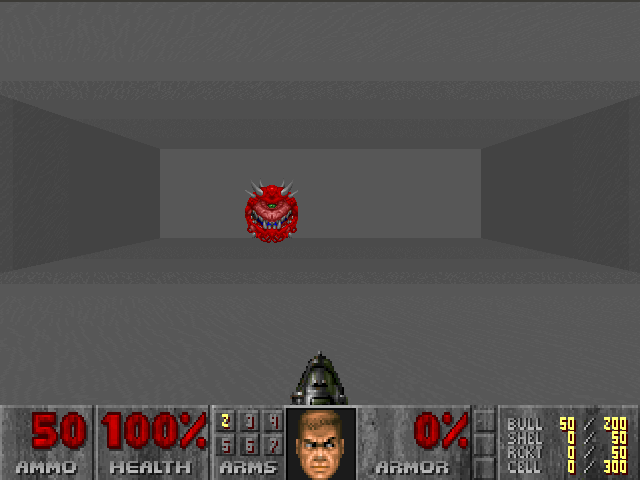
\includegraphics[scale=0.46]{basic.png}
			\caption{Doom gameplay frame from `basic' scenario.}\label{fig:basic}
		\end{figure}

		\paragraph{Motivation}
			Main purpose of this scenario is to show that using VIZIA for Reinforcement Learning from visual input is a feasible idea. The scenario exposes most fundamental mechanics of the game like shooting, movement and delays between actions and reactions of the world.
		
		\paragraph{Description}
			The map is a rectangle with gray walls, ceiling and floor. Agent is spawned along the longer wall, in the center. A red, circular monster is spawned randomly somewhere along the~opposite wall. Agent can only (config) move left, move right and~shoot. A single hit is enough to kill the~monster. Episode ends when the monster is killed or on timeout.
		
		\paragraph{Rewards}
			\begin{itemize}
				\item $+101$ for killing the monster
				\item $-5$ for missing
			\end{itemize}
		
		\paragraph{Suggested configuration}
			\begin{itemize}
				\item living reward = $-1$
				\item available buttons: move left, move right, shoot (attack)
				\item timeout = 300
			\end{itemize}
	\newpage

	\subsection{Deadly Corridor}
		\begin{figure}
			\centering
			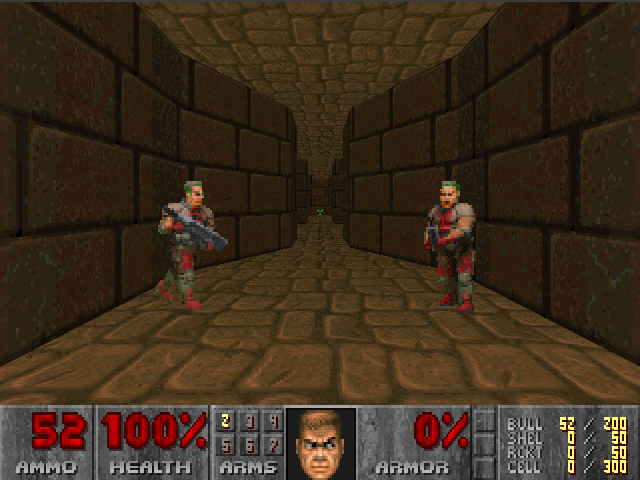
\includegraphics[scale=0.5]{deadly_corridor.png}
			\caption{Doom gameplay frame from `deadly corridor' scenario.}\label{fig:deadly_corridor}
		\end{figure}

		\paragraph{Motivation} 
			The purpose of this scenario is essentially to teach an agent to be a responsible adult with good spacial orientation: focus efforts towards a good direction and be able to sacrifice instant gratification in favor of future benefits and lifespan. Coping with the task requires some degree of spacial orientation and ability to see connection between monsters' presence and deteriorating health which, unattended, results in agent's death.

		\paragraph{Description}
			The map is a corridor with shooting monsters standing along the longer walls (6 monsters in total). Agent is spawned at one end of the corridor and a green vest is placed at the opposite one. Reward is proportional (negative or positive) to change of the distance between the agent and the vest. If agent ignores monsters on the sides and runs straight for the vest he will be killed somewhere along the way. To ensure this behavior \textit{doom\_skill} equal to 5 (config) is needed.

		\paragraph{Rewards}
			\begin{itemize}
				\item $\Delta$x for getting closer to(further from) the vest by $\Delta$x units in the corridor's axis of symmetry.
			\end{itemize}
			
		\paragraph{Suggested configuration}
			\begin{itemize}
				\item available buttons: turn left, turn right, move left, move right, shoot (attack)
				\item timeout = 4200
				\item death penalty = 100
				\item doom skill = 5
				\item available game variables: HEALTH
			\end{itemize}
	\newpage

	\subsection{Defend the Center}\label{subsec:defend_the_center}
		\begin{figure}
			\centering
			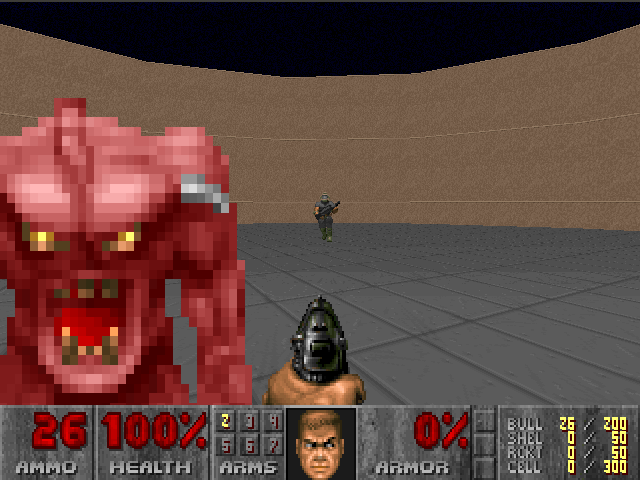
\includegraphics[scale=0.5]{defend_the_center.png}
			\caption{Doom gameplay frame from `defend the center' scenario.}\label{fig:defend_the_center}
		\end{figure}
		\paragraph{Motivation} 
			The purpose of this scenario is to encourage agents to develop some intuition about distances and awareness of potential dangers coming from behind. Obviously, agents should also learn that monsters are sinister and killing them is rewarding, but it is not sufficient. Coincidentally an agent could be expected to learn to impersonate a classical Greek tragic hero: he is doomed to die pitifully (ammunition is finite) regardless of his actions.

		\paragraph{Description}
			The map is a large circle. A player is spawned in the exact center and is allowed to turn and shoot (config). 5 melee-only, monsters are spawned along the wall. Monsters are killed after a single hit. If slain, monsters respawn after some time. Episode ends when the player dies (it is inevitable because of limited ammunition supplies).

		\paragraph{Rewards}
			\begin{itemize}
				\item $+1$ for killing a monster
			\end{itemize}
		
		\paragraph{Suggested configuration}
			\begin{itemize}
				\item death penalty = 1
				\item available buttons: turn left, turn right, shoot (attack)
				\item available game variables: HEALTH, AMMO2(pistol ammo)
			\end{itemize}
	\newpage

	\subsection{Defend the Line}
		\begin{figure}
			\centering
			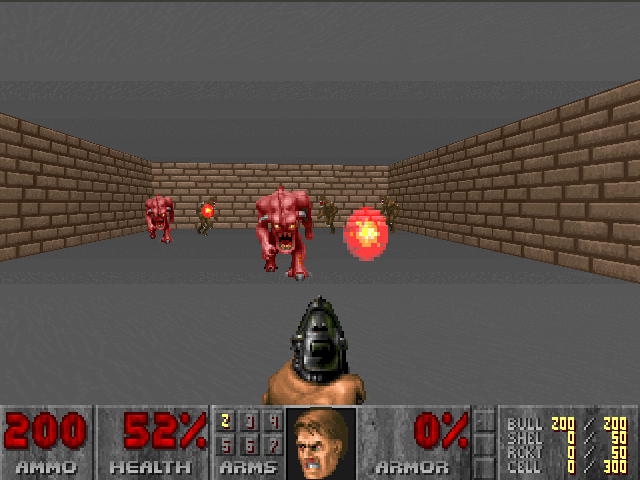
\includegraphics[scale=0.5]{defend_the_line.png}
			\caption{Doom gameplay frame from `defend the line' scenario.}\label{fig:defend_the_line}
		\end{figure}
		\paragraph{Motivation} 
			The purpose of this scenarios is to teach agents risk assessment and basic monster taxonomy by presenting them with monsters of two types: melee fighters and shooters. Agents should be able to recognize that shooters pose more immediate threat than melee monster (unless they are at point blank range). Obviously, agents should also learn that monsters are sinister and killing them is rewarding, however it is not sufficient to perform superbly.
		\paragraph{Description}
			The map is a rectangle. Player is spawned along the longer wall, in the center and is able to turn and shoot(config). 3 melee and 3 shooting monsters are spawned along the opposite wall. Monsters are killed after a single shot, at first. When slain, each monster is respawned after some time and can endure more damage than before. Episode ends when the player dies (it's inevitable because at some point monsters will be too tough to kill).
		\paragraph{Rewards}
			\begin{itemize}
				\item $+1$ for killing a monster
			\end{itemize}

		\paragraph{Suggested configuration}
			\begin{itemize}
				\item available buttons: move left, move right, shoot (attack)
				\item death penalty = 1
				\item available game variables: HEALTH, AMMO2(pistol ammo)
			\end{itemize}
	\newpage

	\subsection{Deathmatch}
		\begin{figure}
			\centering
			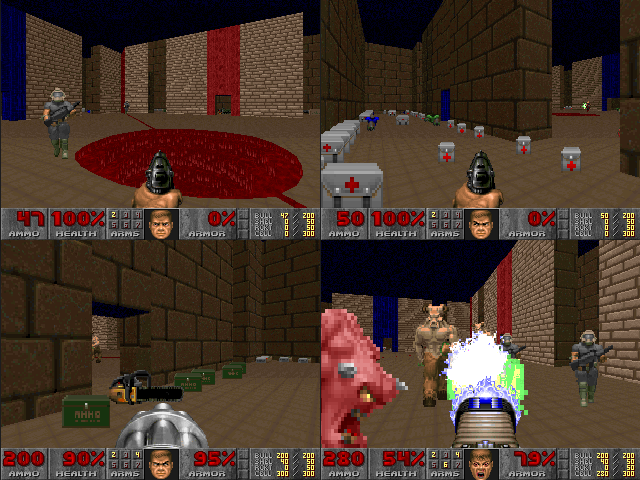
\includegraphics[scale=0.5]{deathmatch.png}
			\caption{4 Doom gameplay frames from `deathmatch' scenario.}\label{fig:deatchmatch}
		\end{figure}
		\paragraph{Motivation} 
	 		This scenario is a fully fledged fight for survival that hopefully requires quite sophisticated cognitive processes. Agent should be able to present effective understanding of many high level concepts as fleeing, surroundings awareness, hiding, camping, resupplying, navigation or changing weapons to survive and kill a significant number of monsters.

		\paragraph{Description}
			The map consists of a square room (hall) of considerable size and 4 small rooms (supply rooms) adjacent to each wall of the hall. 2 supply rooms contain significant quantity of medkits and armors. Other 2 contain (each one) a shotgun, chainsaw, plasma gun, chaingun, rocket launcher and ammunition needed for aforementioned weapons. Agent is spawned in random location inside the hall. After a very short period monsters start spawning in random locations of the hall. Monsters include shooters and melee brawlers. Agent is rewarded for killing monsters. Toughest monsters are less probable to appear and produce greater rewards.
		\paragraph{Rewards}
			\begin{itemize}
				\item $+1/2/3/4/5/10$ for killing a monster (exact value depends on monster type).
			\end{itemize}
		
		\paragraph{Suggested configuration}
			\begin{itemize}
				\item available buttons: all buttons corresponding movement, turning, shooting and weapon change 
				\item timeout = preferred finite value
				\item death penalty = 100
				\item available game variables: HEALTH, ARMOR and all variables connected with weapons and ammo
			\end{itemize}		
	\newpage

	\subsection{Health Gathering}
		\begin{figure}
			\centering
			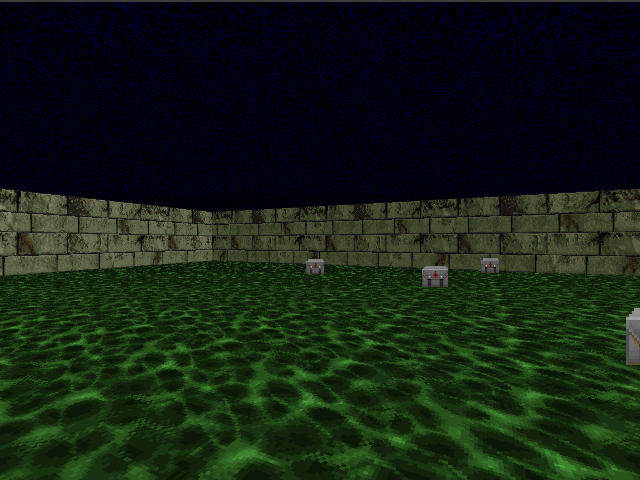
\includegraphics[scale=0.5]{health_gathering.png}
			\caption{Doom gameplay frame from `health gathering' scenario.}\label{fig:health_gathering}
		\end{figure}
		\paragraph{Motivation}
			The purpose of this scenario is to teach an agent that every second of his life is precious and collecting things increases his life expectancy in this brutal world. The agent should be able to see that deteriorating health causes death and how walking into medkits influences his health. It is advisable to equip the agent with some kind of memory because medkits that are directly in front of agent's feet cannot be noticed. In case of developing consciousness agent could also deduce that there is a divine being in the skies that loves him and sends provisions to save him.

		\paragraph{Description}
			The map is a rectangle with green, acidic floor which hurts players periodically. Deadliness of acid depends on skill level. Agent is spawned in the exact center of the map and is able to turn and move forward (config).  Initially there are some medkits uniformly distributed over the map. New medkits fall from the skies periodically. A medkit heals some portion of player's health --- to survive agent needs to pick them up. Episode finishes after player's death or on timeout.

		\paragraph{Suggested configuration}
		\begin{itemize}
			\item living reward = 1
			\item death penalty = 100
			\item available buttons: move left, move right, move forward
			\item timeout = 2100
			\item available game variable: HEALTH
		\end{itemize}
	\newpage

	\subsection{My Way Home}
		\begin{figure}
			\centering
			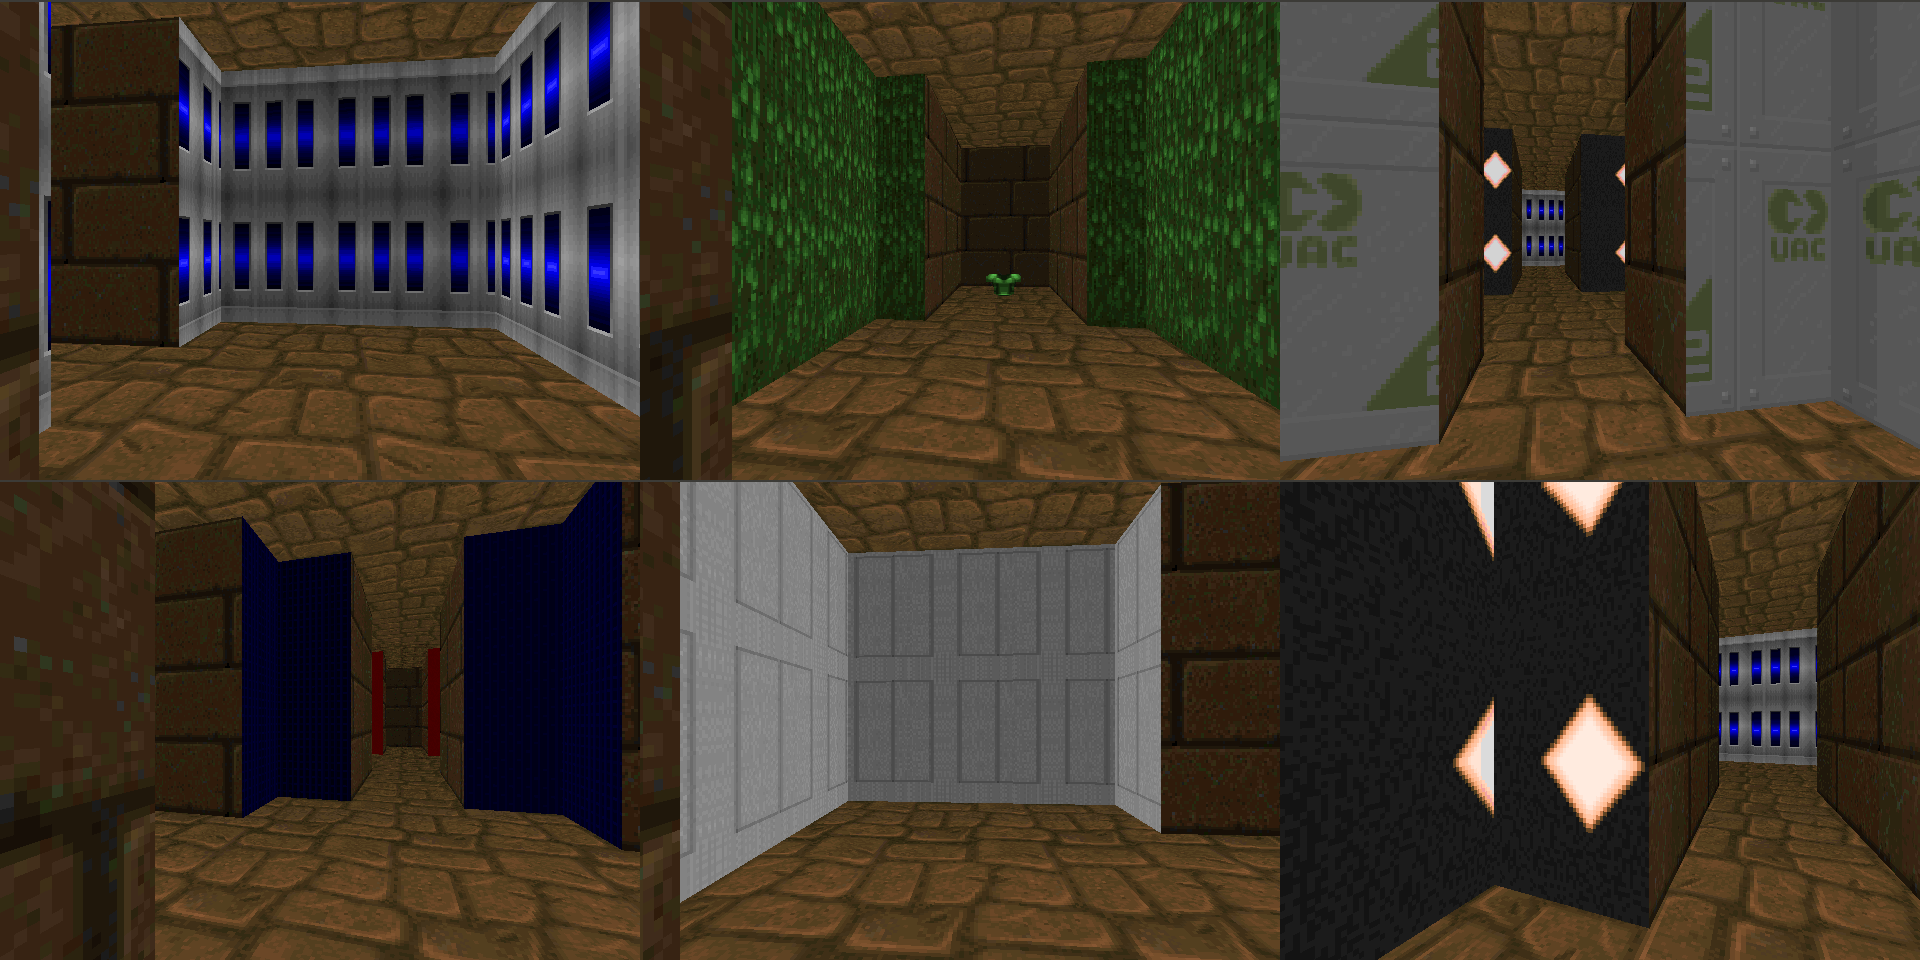
\includegraphics[scale=0.22]{my_way_home.png}
			\caption{6 Doom gameplay frames from `my way home' scenario.}\label{fig:my_way_home}
		\end{figure}
		\paragraph{Motivation} 
			The purpose of this scenario is to teach the agent how to navigate in a labyrinth-like environment and reach his ultimate goal (and learn what the goal actually is). Agent should learn to determine his position in the maze and to navigate accordingly.

		\paragraph{Description}
			The map is a series of small rooms interconnected with each other by short passages and a single dead end corridor. Each room has a different color. A green vest is placed in one of the rooms (the same room every time). Player is spawned in randomly chosen room facing a random direction. Episode ends when the vest is reached or on timeout.
		\paragraph{Rewards}

		\begin{itemize}
			\item $+1$ for reaching the vest
		\end{itemize}
		
		\paragraph{Suggested configuration}
		\begin{itemize}
			\item living reward = $-0.0001$
			\item available buttons: move left, move right, shoot (attack)
			\item timeout = 2100
		\end{itemize}
	\newpage

	\subsection{Predict Position}
		\begin{figure}
			\centering
			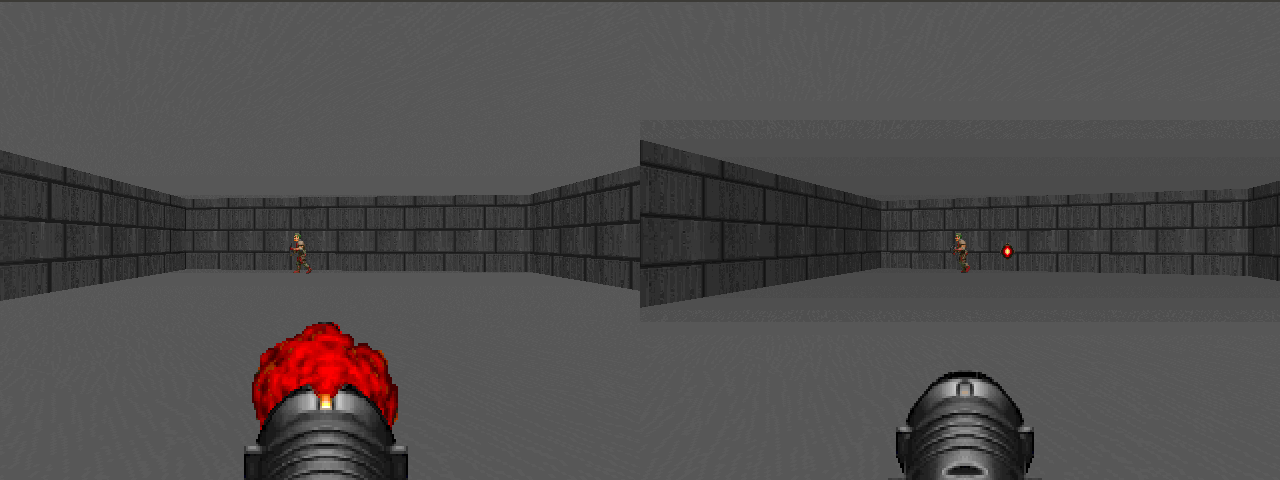
\includegraphics[scale=0.32]{predict_position.png}
			\caption{2 Doom gameplay frames from `predict position' scenario.}\label{fig:predict_position}
		\end{figure}
		\paragraph{Motivation} 
			The purpose of the scenario is to teach agents to synchronize missile weapon shots (involving a significant delay between shooting and hitting) with target movements. Agent should be able to shoot so that missile and monster meet each other.

		\paragraph{Description}
			The map is a rectangle room. Agent is spawned along the longer wall, in the center and is allowed to turn and shoot(config). A monster is spawned randomly somewhere along the opposite wall and walks between left and right corners along the wall. Player is equipped with a rocket launcher and a single rocket. Episode ends when the missile hits the monster (or a wall) or on timeout.
		\paragraph{Rewards}
		\begin{itemize}
			\item $+1$ for killing the monster
		\end{itemize}
		
		\paragraph{Suggested configuration}
		\begin{itemize}
			\item living reward = $-0.0001$
			\item available buttons: turn left, turn right, shoot (attack)
			\item timeout = 300
		\end{itemize}
	\newpage

	\subsection{Take Cover}
		\begin{figure}
			\centering
			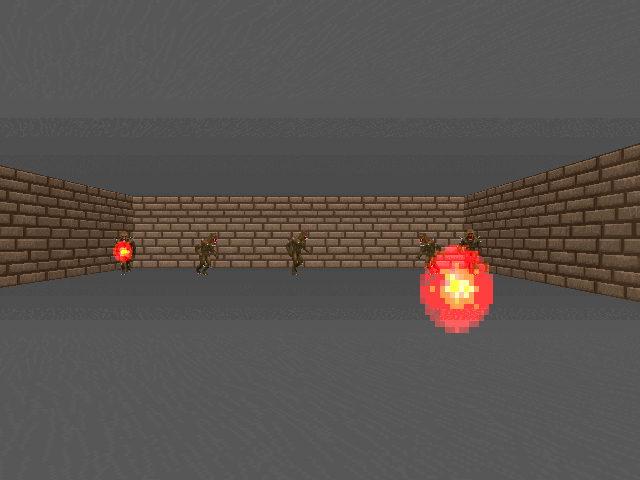
\includegraphics[scale=0.5]{take_cover.png}
			\caption{Doom gameplay frame from `take cover' scenario.}
		\end{figure}
		\paragraph{Motivation} 
			The purpose of this scenario is to teach agents to link incoming missiles with their estimated lifespan. Agents should learn that being hit means a decrease in health and this in turn leads to death that is most undesirable. In effect agents should learn how to avoid missiles.

		\paragraph{Description}
			Map is a rectangle. Player is spawned along the longer wall, in the center. A couple of fireball-spitting monsters are spawned randomly somewhere along the opposite wall and try to kill the player with fireballs. The player has no weapon and can only move sideways (config). More monsters appear with time. Episode ends when player dies which is inevitable. In case the agent was expected to reach super-human performance some timeout(config) might be suggested as death may not be inevitable.

		\paragraph{Suggested configuration}
		\begin{itemize}
			\item living reward = 1
			\item death penalty = 100
			\item 2 available buttons: move left, move right
		\end{itemize}
	\newpage

\section{Creating scenarios}\label{sec:creating_scenarios}
	This section is not intended as a reference manual for Action Code Script (ACS) or map creation thus covers only subjects directly relevant to interfacing between Doom game engine and VIZIA.


	\subsection{Fixed Point Numbers}\label{subsec:fixed_point}
		ACS does not support floating point numbers, however fixed point numbers are implemented using integers. By adding a decimal point the compiler is force to treat \emph{int} variable as a fixed point number so for instance `1' will be treated as an integer whereas `1.0' as a fixed point numeral. Mixing integers and fixed point numbers is allowed but will produce unexpected results if performed unknowingly. For more detailed information consult ZDoom Wiki Webpage\cite{zdoom-wiki}.

	\subsection{Global Variables}\label{subsec:global_variable}
		ACS provides a special type of variables called \emph{global~variables} that are seen by VIZIA API as game variables (see Section \ref{subsec:gamevar}) named USER<X>. Global variables behave the same as ordinary variables but need to be declared in global scope and in a slightly different way:
		\begin{clinee}
global int <X>:reward;
		\end{clinee}
		Where <X> denotes the ordinal number of the variable.
		
	\subsection{Rewards}
		In order to support the rewarding mechanism, it is necessary to utilize global variable 0 in the ACS script. Name given to the variable does not matter. The value of the variable represents total reward accumulated throughout the whole episode so in order to give a reward for a specific action it is needed to increase global variable 0 by the desired value not to assign it. VIZIA treats the reward global variable as a fixed point number(see \ref{subsec:fixed_point}).

	\subsection{Advices}
		This section shows code snippets showing how we achieved some ACS scripting behaviors that may prove useful. The code snippets intend to be relatively self-explanatory and assume knowledge of the very basics of ACS scripting and capability of reading documentation to make sense of used functions. For documentation and more detailed information consult ZDoom Wiki Webpage\cite{zdoom-wiki}.

		\subsubsection*{Ending an Episode}

			\begin{clinee}
Exit_Normal(0);
			\end{clinee}
		\subsubsection*{Reward for Killing a Monster} This snippet is also useful for triggering any event after killing a monster or collecting an item.
			\begin{clinee}
script 123 (void)
{
	reward = reward + 1;
}
SetThingSpecial(MONSTER_TID, ACS_ExecuteAlways, 123);
			\end{clinee}
\subsubsection*{Friendly Monster}
			\begin{clinee}
Thing_Hate (MONSTER_TID, SOME_UNUSED_TID, 6);
			\end{clinee}
		\subsubsection*{Stationary Monster}
			\begin{clinee}
SetActorProperty(MONSTER_TID, APROP_Speed, 0);
			\end{clinee}
		\subsubsection*{Single Hit Monster}
			\begin{clinee}
SetActorProperty(MONSTER_TID, APROP_Health, 1);
			\end{clinee}
		\subsubsection*{Self-replenishing Ammo}
		Note that this can also be achieved by changing ZDoom's configuration but these changes are persistent.
			\begin{clinee}
script 2 ENTER
{   
    while(1)
    {
        delay(1);
        GiveInventory("Clip", 1 );
    }
}
			\end{clinee}
		\subsubsection*{Disappearing Corpses}
			\begin{clinee}
script 234 (int TID)
{
	Thing_Remove(TID);
}
SetThingSpecial(MONSTER_TID, ACS_ExecuteAlways, 234, MONSTER_TID);
			\end{clinee}
\chapter{Reinforcement Deep Learning Experiment}\label{ch:experiment}

\section{Goal of the Experiment}
The main purpose of the experiment is to show that reinforcement learning from visual input is possible using VIZIA Environment. 	
Additionally, the experiment tries to investigate how skipping varying number of frames influences learning process.

\section{Experiment's Design}
During the experiment, agents with varying \emph{skiprates} are to be tested. We define \emph{skiprate} as the number of game frames that are skipped(ignored) by agent for every frame that is processed. Skipping a frame is accomplished with \emph{makeAction} method with tics argument set to skiprate (see Section \ref{subsec:runtime_methods}) so rewards are accumulated and the chosen action is extended for the duration of skipped frames. Skiprate values of 0,1,2,3,4,5~and~7 are evaluated in the experiment. 

Every agent is to run 80 epochs. Each epoch requires performing 5000 learning steps that involve performing an action (observing a transition) and running a learning update. After the learning portion of each epoch, 100 random test episodes are conducted and mean score is used for assessment.  

\section{Tested Agent's Design}
	The agent is heavily inspired by Google DeepMind Atari DQN \cite{mnih-dqn-2015}\cite{mnih-atari-2013} and is conceptually very similar to the aforementioned algorithm. Game is modeled as a Markov Decision Process and Q-learning \cite{watkins:mlj92} is used to reach the optimal policy. $\epsilon$-greedy policy with linear $\epsilon$ decay is used to choose actions. Additionally, a technique called experience replay \cite{mnih-dqn-2015} is applied. A state is represented by only the most recent image therefore agents have no memory. A Convolutional Neural Network is used for approximation of Q-values and it is trained with Backpropagation Algorithm \cite{lecun-98b} using Stochastic Gradient Descent with mini-batches. An agent is implemented in Python and uses Theano \cite{Bastien-Theano-2012}\cite{bergstra+al:2010-scipy} and Lasagne \cite{sander_dieleman_2015_27878} libraries for neural networks. Neural network's forward and backward passes are computed on GPU whereas the rest of the code runs on the CPU.

\newpage
\section{Experimental Setup} 
	\subsection{Operating System and Hardware}
	\begin{description}
		\item[Operating System] Linux Mint 17 x86\_64, kernel 3.13.0-24-generic
		\item[CPU] Intel Core i7-4790, 4x4GHz
		\item[GPU] GeForce GTX 970, 1664 CUDA cores, 4GB RAM
	\end{description}

	\subsection{Game Settings}
		The experiment uses the simplest scenario from the pool, that is the `basic' scenario (see \ref{subsec:basic}). State is represented by 3-channel image (RGB) with resolution of 60 by 45 pixels.

	\subsection{Neural Network Architecture}
		\begin{figure}
			\centering
			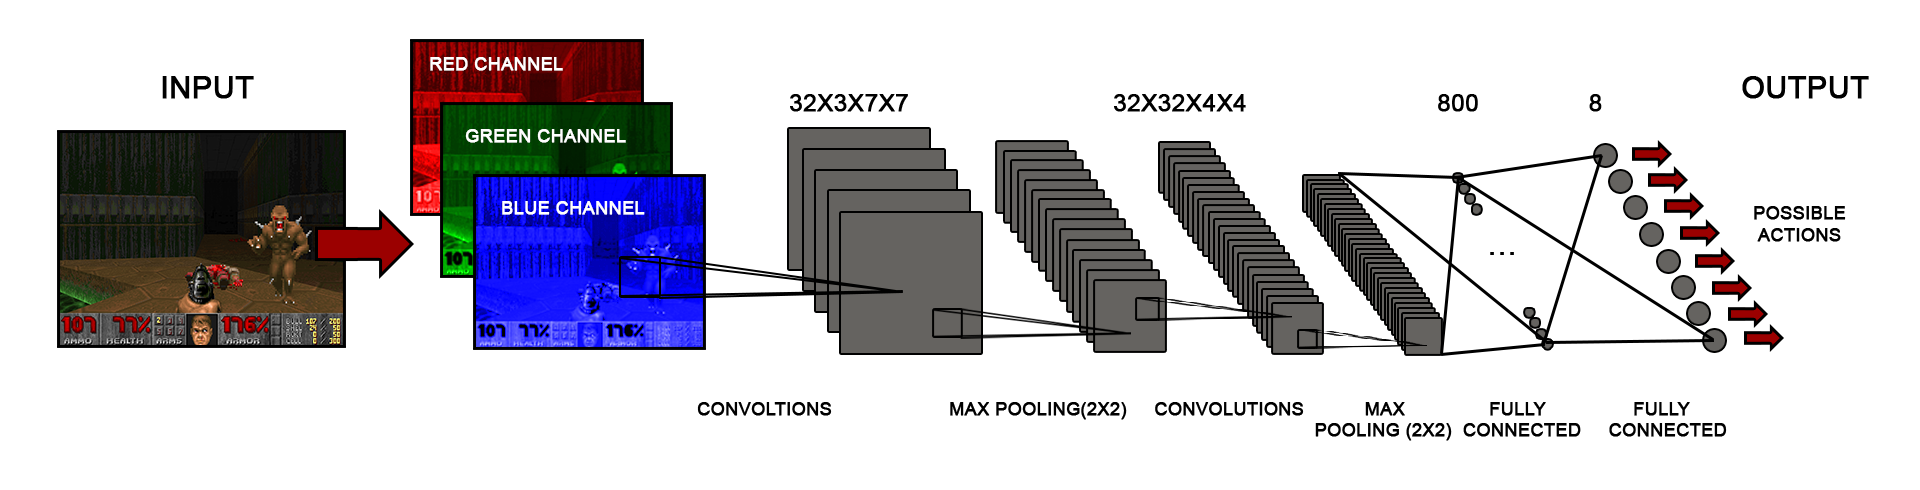
\includegraphics[scale=0.25]{net_diagram.png}
			\caption{Schematic illustration of neural network used for the experiment.}\label{fig:network}
		\end{figure}
		 The network used in the experiment consists of two convolutional layers with 32 square filters (7 and 4 pixels wide) each connected to a max-pooling layer with poolsize equal to 2 and rectifier linear units. Convolutional layers are followed by a fully connected layer with 800 leaky rectified linear units and output layer with 8 linear units corresponding to 8 available actions (combinations of 3 available buttons). The architecture used is rather modest, compared to the ones used for other tasks recently.
	
	\subsection{Hyper Parameters}
		\begin{itemize}
		\item $\gamma$ (discount factor) = 0.99
		\item learning rate = 0.01
		\item mini-batch size = 40
		\item initial $\epsilon$ = 1.0
		\item final $\epsilon$ = 0.1
		\item steps after which $\epsilon$ decay will start = 100000
		\item steps to fully decrease $\epsilon$ = 100000
		\item replay memory  capacity = 10000
		\end{itemize}
	

\section{Results}
		\begin{figure}
			\centering
			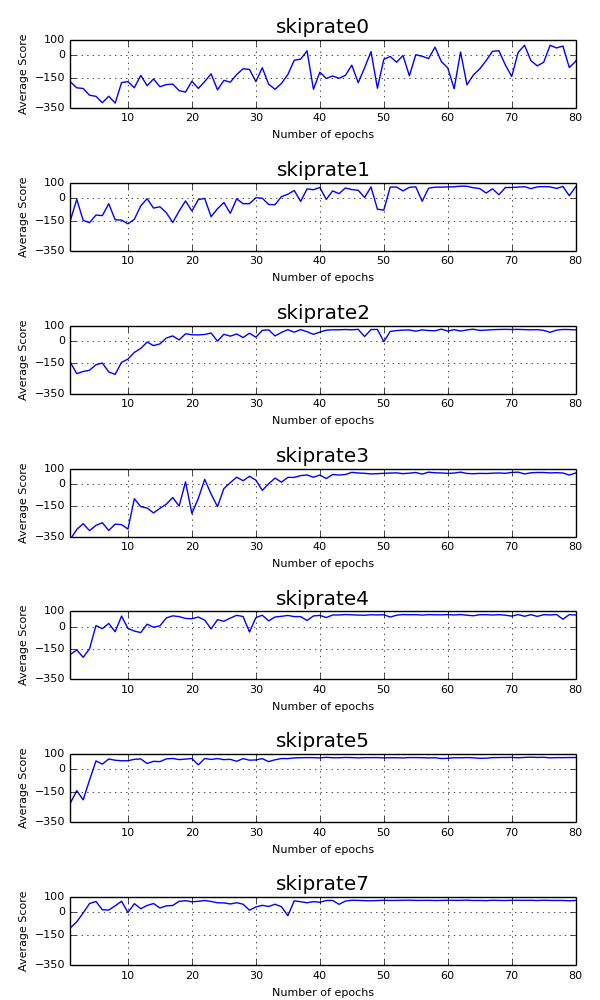
\includegraphics{results.png}
			\caption{Graphs showing mean performance of tested agent with different skip values throughout 80 learning epochs.}\label{fig:results}
		\end{figure}
	\subsection{Numerical Issues}
		In case of 0 skiprate a major numerical problem was encountered. Estimated Q-values usually ($\approx$50\% of runs) rapidly grew to infinite values (in the first epoch) which prevented further learning. Quite unexpectedly, increasing resolution from 60x45 to 120x90 eliminated the problem at the cost of longer learning time. Faulty code would be an obvious explanation, however no apparent error has been found yet therefore a conceptually oriented mechanism is also to be considered. It is hypothesized that combination of zero skiprate and low resolution may produce state transitions that incorporate barely distinguishable states. As a consequence each update would significantly inflate Q-values for each state and rapidly reach infinity. Although changing the resolution seemed to solve the problem, it is not a satisfying solution and one based on mechanics of Q-learning itself would be much more desirable.

		Skiprate 0 setting was tested for both resolutions, however the agent with increased resolution was considered separately (see Figure \ref{fig:results_skiprate0}). Due to high number of epochs required to get fairly satisfying results with zero skiprate and increased resolution, learning was continued for further 270 epochs to see if it would follow the trend as expected.

	\subsection{Learning Quality}
		As seen in Figure \ref{fig:results}, all agents reached estimated maximum average score of $\approx$80 or showed trend towards achieving similar value. Watching agents play the scenario proved that agents in fact behave very reasonably. They move towards the target and shoot when it appears in front of them. Occasionally agents fire marginally too soon or stay idle (first available action) throughout whole episode. 
		
	\subsection{Skiprate Influence}
			
			
		\subsubsection*{Learning speed} 

			\begin{table}
				\begin{center}
					\begin{tabular}{ |c | c |}
						\hline
						Skiprate & Average epoch duration [s] \\ \hline
						0 & 51.79 \\ \hline
						1 & 51.83 \\ \hline
						2 & 52.84 \\ \hline
						3 & 53.84 \\ \hline
						4 & 52.88 \\ \hline
						5 & 53.15 \\ \hline
						7 & 53.12 \\ \hline
					\end{tabular}
				\end{center}
				\caption{Influence of skiprate on processing time for resolution of 60X45}\label{tab:time_results}
			\end{table}
			As seen in the Figure \ref{fig:results} higher skiprate leads to quicker (in terms of learning steps) and smoother learning, which was expected as higher skiprate makes consequences of actions more immediate and easier to notice. However, it must be pointed out that epoch's duration slightly increases with raising skiprate (see Table \ref{tab:time_results}). Obviously, such behavior was anticipated because Doom engine has to process skiprate as many frames (which we skip) for a single learning step (action). Additionally, higher skiprate results in episodes being shorter (because we skip most of frames) which increases overhead associated with episode restarts (restarts are more frequent). 

		\subsubsection*{Score}
			\begin{table}
				\begin{center}
					\begin{tabular}{ |l || c | r |}
						\hline
						Skiprate & Best epoch score & Mean of 10 best epochs \\ \hline
						0 & 69.18 $\pm$ 50.24 & 60.97 \\ \hline
						1 & 77.84 $\pm$ 22.71 & 76.19 \\ \hline
						2 & 79.35 $\pm$ 20.68 & 77.91 \\ \hline
						3 & 80.98 $\pm$ 22.89 & 78.69 \\ \hline
						4 & 81.8 $\pm$ 17.99 & 80.75 \\ \hline
						5 & 81.32 $\pm$ 19.47 & 80.16 \\ \hline
						7 & 81.08 $\pm$ 18.9 & 80.5 \\ \hline
					\end{tabular}
				\end{center}
				\caption{Influence of skiprate on highscores achieved in 80 epochs.}\label{tab:results}
			\end{table}
			It was also anticipated that higher skiprate could slightly lower scores due to the lack of small-grained control. As seen in Table \ref{tab:results}, it is exactly the opposite. It is doubtful whether too short training is the culprit of this trend, since most of agents reach significant stability in 80 epochs and do not appear to be able to ever transcend achieved highscores (at least for skiprates $\geq$ 2). What is more, it was observed that agents with higher skiprates were less prone to irrational behaviors like staying idle or going the opposite way which may coincide with much smoother learning. However, it is hypothesized that careful fine-tuning of hyper parameters could positively influence learning rate and smoothness. 

			Learning process was especially fuzzy for zero skiprate with increased resolution (see Figure \ref{fig:results_skiprate0}) but it appears that it was slowly converging to the optimum and intensity of occasional terrible-performance episodes was fading. Further learning (preferably with lowered learning rate) would be necessary to confirm the hypothesis.
	
	\begin{figure}
		\centering
		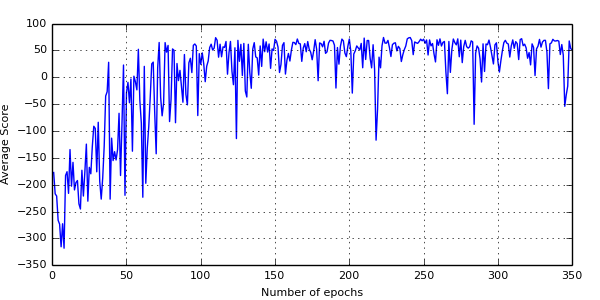
\includegraphics{results_skiprate0.png}
		\caption{Graphs showing mean performance of agent with zero skiprate and resolution 120x90 throughout 350 learning epochs.}\label{fig:results_skiprate0}
	\end{figure}

	
\chapter{Conclusions}\label{ch:conclusions}
	It is strongly believed that Vizia project has been carried out successfully and provides a stable and lightweight tool for research on reinforcement learning in 3-dimensional environment. API is equipped with multiple useful modes (see Section \ref{sec:architecture_modes}) which allow apprenticeship learning, multiplayer game and naturally ordinary learning in the reinforcement learning paradigm. What is more, different modes enable researchers to decide if full control over game engine's processing is needed or if it is the game that should set the pace. Furthermore, the mechanism of scenarios has been employed with much success, making it very easy to create custom research conditions. Section \ref{sec:performance} shows that VIZIA's performance is satisfactory and conducted experiment (see Chapter \ref{ch:experiment}) proves that using VIZIA is viable in practice. 

\section{Achieved Goals}
	\begin{itemize}
		\item Enforcement of full control over 3D engine processing.
		\item Satisfactory performance and stability.
		\item Custom scenarios support.
		\item Spectator mode allowing apprenticeship learning.
		\item Support for asynchronous multiplayer.
		\item Bindings for Python and Java.
		\item Support for depth buffer.
	\end{itemize}

\section{Future Work}
	\begin{itemize}
		\item Lua binding.
		\item Better Windows and Mac support.
		\item Support for multiplayer mode in synchronous modes.
	\end{itemize}


% Bibliography (books, articles) starts here.
\bibliographystyle{plain}{\raggedright\sloppy\small\bibliography{bibliography}}

% All appendices and extra material, if you have any.
\cleardoublepage\appendix%
%
\chapter{GitHub}
The thesis and VIZIA framework are available on the github server: \\
\url{https://github.com/Marqt/Vizia/}


\chapter{Building}
\section{Prerequisites}
\begin{itemize}
\item preferably Linux
\item cmake
\item make
\item gcc 4.??
\item Boost 
\item Python 2.6+ with Numpy and Boost.Python (for pyhon binding)
\item Java compiler (for Java binding)
\end{itemize}
\section{Before Building}
	In addition to prerequisites mentioned above, the following packages need to be install to build Zdoom itself:
	\begin{description}
		\item[Debian/Ubuntu:] \hfill \\
		sudo apt-get install build-essential zlib1g-dev libsdl2-dev libjpeg-dev nasm tar libbz2-dev libgtk2.0-dev cmake git libfluidsynth-dev libgme-dev libopenal-dev timidity
		\item[Fedora:] \hfill \\
		yum install gcc-c++ make zlib-devel SDL2-devel libjpeg-turbo-devel nasm tar bzip2-devel gtk2-devel cmake git fluidsynth-devel game-music-emu-devel	openal-soft-devel timidity++
		\item[Arch linux:] \hfill \\
		pacman -S --needed gcc make zlib sdl2 libjpeg-turbo nasm tar bzip2 gtk2 cmake git fluidsynth libgme fmodex openal timidity++
		\item[openSUSE:] \hfill \\
		zypper install gcc-c++ make zlib-devel libSDL2-devel libjpeg-devel nasm tar libbz2-devel gtk2-devel cmake git fluidsynth-devel libgme-devel openal-soft-devel timidity
	\end{description}
\section{Compilation}
To compile Vizia run this commands 
	\begin{lstlisting}
cmake -DCMAKE_BUILD_TYPE=Release
make all
	\end{lstlisting}
\chapter{Methods and Structures Handout}
\section{Methods}


\begin{clinee}
DoomGame::~DoomGame();
\end{clinee}


\begin{clinee}
bool DoomGame::init();
\end{clinee}


\begin{clinee}
bool DoomGame::loadConfig(std::string configFilePath);
\end{clinee}


\begin{clinee}
void DoomGame::addAvailableButton(Button button);
\end{clinee}

\begin{clinee}
void DoomGame::setButtonMaxValue(Button button, int maxValue);
\end{clinee}


\begin{clinee}
void DoomGame::addAvailableButton(Button button, int maxValue);
\end{clinee}


\begin{clinee}
void DoomGame::clearAvailableButtons();
\end{clinee}


\begin{clinee}
void DoomGame::addAvailableGameVariable(GameVariable var);
\end{clinee}


\begin{clinee}
void DoomGame::clearAvailableGameVariables();
\end{clinee}
	

\begin{clinee}
void DoomGame::addCustomGameArg(std::string arg);
\end{clinee}


\begin{clinee}
void DoomGame::clearCustomGameArgs();
\end{clinee}


\begin{clinee}
void DoomGame::setMode(Mode mode);
\end{clinee}
	

\begin{clinee}
void DoomGame::setDoomEnginePath(std::string path);
\end{clinee}


\begin{clinee}
void DoomGame::setDoomGamePath(std::string path);
\end{clinee}


\begin{clinee}
void DoomGame::setDoomScenarioPath(std::string path);
\end{clinee}


\begin{clinee}
void DoomGame::setDoomConfigPath(std::string path);
\end{clinee}


\begin{clinee}
void DoomGame::setDoomMap(std::string map);
\end{clinee}
	

\begin{clinee}      
void DoomGame::setDoomSkill(int skill);
\end{clinee}
	

\begin{clinee}    
void DoomGame::setEpisodeStartTime(unsigned int tics);
\end{clinee}


\begin{clinee}
void DoomGame::setEpisodeTimeout(unsigned int tics);
\end{clinee}


\begin{clinee}
void DoomGame::setLivingReward(double livingReward);
\end{clinee}


\begin{clinee}
void DoomGame::setDeathPenalty(double deathPenalty);
\end{clinee}
	

\begin{clinee}
void DoomGame::setScreenResolution(ScreenResolution resolution);
\end{clinee}


\begin{clinee}
void DoomGame::setScreenFormat(ScreenFormat format);
\end{clinee}
	

\begin{clinee}       
void DoomGame::setRenderHud(bool hud);
\end{clinee}


\begin{clinee}  
void DoomGame::setRenderWeapon(bool weapon);
\end{clinee}


\begin{clinee}  
void DoomGame::setRenderCrosshair(bool crosshair);
\end{clinee}


\begin{clinee}  
void DoomGame::setRenderDecals(bool decals);
\end{clinee}


\begin{clinee}  
void DoomGame::setRenderParticles(bool particles);
\end{clinee}


\begin{clinee}
void DoomGame::setWindowVisible(bool visibility);
\end{clinee}


\begin{clinee}
void DoomGame::setConsoleEnabled(bool console);
\end{clinee}
	

\subsection{Runtime Methods}\label{subsec:runtime_methods}
	

\begin{clinee}
void DoomGame::newEpisode();
\end{clinee}


\begin{clinee}
	void DoomGame::setAction(std::vector<int> const &actions);
\end{clinee}


\begin{clinee}
	void DoomGame::advanceAction(unsigned int tics, bool stateUpdate, bool renderOnly);
\end{clinee}


\begin{clinee}
	void DoomGame::advanceAction(unsigned int tics);
\end{clinee}


\begin{clinee}
	void DoomGame::advanceAction();
\end{clinee}


\begin{clinee}
	void DoomGame::advanceAction(unsigned int tics, bool stateUpdate, bool renderOnly);
\end{clinee}


\begin{clinee}
	double DoomGame::getLastReward();
\end{clinee}


\begin{clinee}
	double DoomGame::makeAction(std::vector<int> const &actions, unsigned int tics);
\end{clinee}

   
\begin{clinee}
	double DoomGame::makeAction(std::vector<int> const &actions);
\end{clinee}


\begin{clinee}
	DoomGame::State DoomGame::getState();
\end{clinee}


\begin{clinee}
	std::vector<int> DoomGame::getLastAction();
\end{clinee}


\begin{clinee}
	uint8_t * const getGameScreen();
\end{clinee}


\begin{clinee}
	int DoomGame::getGameVariable(GameVariable var);
\end{clinee}


\begin{clinee}
	double DoomGame::getSummaryReward();
\end{clinee}


\begin{clinee}
	bool DoomGame::isNewEpisode();
\end{clinee}


\begin{clinee}
	bool DoomGame::isEpisodeFinished();
\end{clinee}


\begin{clinee}
	void DoomGame::setSeed(unsigned int seed);
\end{clinee}


\begin{clinee}
	void DoomGame::close();
\end{clinee}


\begin{clinee}
	bool DoomGame::isRunning();
\end{clinee}


\begin{clinee}
	void DoomGame::sendGameCommand(std::string cmd);
\end{clinee}


\subsection{Query Methods}


\begin{clinee}
int DoomGame::getAvailableButtonsSize();
\end{clinee}

\begin{clinee}
int DoomGame::getAvailableGameVariablesSize();
\end{clinee}

\begin{clinee}
Mode DoomGame::getMode();
\end{clinee}

\begin{clinee}
double DoomGame::getLivingReward();
\end{clinee}

\begin{clinee}
double DoomGame::getDeathPenalty();
\end{clinee}

\begin{clinee}
unsigned int DoomGame::getEpisodeStartTime();
\end{clinee}

\begin{clinee}
unsigned int DoomGame::getEpisodeTimeout();
\end{clinee}

\begin{clinee}
unsigned int DoomGame::getEpisodeTime();
\end{clinee}

\begin{clinee}
int DoomGame::getScreenWidth();
\end{clinee}

\begin{clinee}
int DoomGame::getScreenHeight();
\end{clinee}

\begin{clinee}
int DoomGame::getScreenChannels();
\end{clinee}

\begin{clinee}
size_t DoomGame::getScreenPitch();
\end{clinee}

\begin{clinee}
size_t DoomGame::getScreenSize();
\end{clinee}

\begin{clinee}
ScreenFormat DoomGame::getScreenFormat();
\end{clinee}

\begin{clinee}
unsigned int DoomGame::getSeed();
\end{clinee}

\begin{clinee}
int DoomGame::getButtonMaxValue(Button button);
\end{clinee}

\section {Utility Functions}


\begin{clinee}
unsigned int DoomTics2Ms(unsigned int tics);
\end{clinee}


\begin{clinee}
unsigned int Ms2DoomTics(unsigned int ms);
\end{clinee}


\begin{clinee}
double DoomFixedToDouble(int doomFixed);
\end{clinee}


\section{Structures and Enumerations}\label{sec:appendix_structs_and_enums}
\subsection{State}

	
\begin{clinee}
	struct State {
	    unsigned int number; 
	    std::vector<int> gameVariables;
	    uint8_t * imageBuffer;
	};
\end{clinee}

\subsection{Mode}\label{subsec:mode}

\paragraph{Modes:}

\begin{itemize}
	\item PLAYER
	\item SPECTATOR
	\item ASYNC\_PLAYER 
	\item ASYNC\_SPECTATOR 
\end{itemize}

\subsection{ScreenFormat}\label{subsec:screenformat}


\textbf{ScreenFormats:}
\begin{itemize}
     \item CRCGCB 
     \item CRCGCBDB
     \item RGB24
     \item RGBA32
     \item ARGB32
     \item CBCGCR
     \item CBCGCRDB
     \item BGR24
     \item BGRA32
     \item ABGR32
     \item GRAY8
     \item DEPTH\_BUFFER8
     \item DOOM\_256\_COLORS8
\end{itemize}
\subsection{ScreenResolution} \label{subsec:screenresolution}


\textbf{ScreenResolutions:}
\begin{itemize}
    \item RES\_40X30
    \item RES\_60X45
    \item RES\_80X50
    \item RES\_80X60
    \item RES\_100X75
    \item RES\_120X75
    \item RES\_120X90
    \item RES\_160X100
    \item RES\_160X120
    \item RES\_200X120
    \item RES\_200X150
    \item RES\_240X135
    \item RES\_240X150
    \item RES\_240X180
    \item RES\_256X144
    \item RES\_256X160
    \item RES\_256X192
    \item RES\_320X200
    \item RES\_320X240
    \item RES\_400X225
    \item RES\_400X300
    \item RES\_480X270
    \item RES\_480X360
    \item RES\_512X288
    \item RES\_512X384
    \item RES\_640X360
    \item RES\_640X400
    \item RES\_640X480
    \item RES\_720X480
    \item RES\_720X540
    \item RES\_800X450
    \item RES\_800X480
    \item RES\_800X500
    \item RES\_800X600
    \item RES\_848X480
    \item RES\_960X600
    \item RES\_960X720
    \item RES\_1024X576
    \item RES\_1024X600
    \item RES\_1024X640
    \item RES\_1024X768
    \item RES\_1088X612
    \item RES\_1152X648
    \item RES\_1152X720
    \item RES\_1152X864
    \item RES\_1280X720
    \item RES\_1280X854
    \item RES\_1280X800
    \item RES\_1280X960
    \item RES\_1280X1024
    \item RES\_1360X768
    \item RES\_1366X768
    \item RES\_1400X787
    \item RES\_1400X875
    \item RES\_1400X1050
    \item RES\_1440X900
    \item RES\_1440X960
    \item RES\_1440X1080
    \item RES\_1600X900
    \item RES\_1600X1000
    \item RES\_1600X1200
    \item RES\_1680X1050
    \item RES\_1920X1080
    \item RES\_1920X1200
    \item RES\_2048X1536
    \item RES\_2560X1440
    \item RES\_2560X1600
    \item RES\_2560X2048
    \item RES\_2880X1800
    \item RES\_3200X1800
    \item RES\_3840X2160
    \item RES\_3840X2400
    \item RES\_4096X2160
    \item RES\_5120X2880
\end{itemize}

\subsection{GameVariable} \label{subsec:gamevar}


\textbf{Game Variables:}
\begin{itemize}
    \item KILLCOUNT
    \item ITEMCOUNT
    \item SECRETCOUNT
    \item FRAGCOUNT
    \item HEALTH
    \item ARMOR
    \item DEAD
    \item ON\_GROUND
    \item ATTACK\_READY
    \item ALTATTACK\_READY
    \item SELECTED\_WEAPON
    \item SELECTED\_WEAPON\_AMMO
    \item AMMO0
    \item AMMO1
    \item AMMO2
    \item AMMO3
    \item AMMO4
    \item AMMO5
    \item AMMO6
    \item AMMO7
    \item AMMO8
    \item AMMO9
    \item WEAPON0
    \item WEAPON1
    \item WEAPON2
    \item WEAPON3
    \item WEAPON4
    \item WEAPON5
    \item WEAPON6
    \item WEAPON7
    \item WEAPON8
    \item WEAPON9
    \item USER1
    \item USER2
    \item USER3
    \item USER4
    \item USER5
    \item USER6
    \item USER7
    \item USER8
    \item USER9
    \item USER10
    \item USER11
    \item USER12
    \item USER13
    \item USER14
    \item USER15
    \item USER16
    \item USER17
    \item USER18
    \item USER19
    \item USER20
    \item USER21
    \item USER22
    \item USER23
    \item USER24
    \item USER25
    \item USER26
    \item USER27
    \item USER28
    \item USER29
    \item USER30
\end{itemize}

\subsection{Button} \label{subsec:button}


\textbf{Buttons:}
\begin{itemize}
    \item ATTACK
    \item USE
    \item JUMP
    \item CROUCH
    \item TURN180
    \item ALTATTACK
    \item RELOAD
    \item ZOOM
    \item SPEED
    \item STRAFE
    \item MOVE\_RIGHT
    \item MOVE\_LEFT
    \item MOVE\_BACKWARD
    \item MOVE\_FORWARD
    \item TURN\_RIGHT
    \item TURN\_LEFT
    \item LOOK\_UP
    \item LOOK\_DOWN
    \item MOVE\_UP
    \item MOVE\_DOWN
    \item LAND
    \item SELECT\_WEAPON1
    \item SELECT\_WEAPON2
    \item SELECT\_WEAPON3
    \item SELECT\_WEAPON4
    \item SELECT\_WEAPON5
    \item SELECT\_WEAPON6
    \item SELECT\_WEAPON7
    \item SELECT\_WEAPON8
    \item SELECT\_WEAPON9
    \item SELECT\_WEAPON0
    \item SELECT\_NEXT\_WEAPON
    \item SELECT\_PREV\_WEAPON
    \item DROP\_SELECTED\_WEAPON
    \item ACTIVATE\_SELECTED\_ITEM
    \item SELECT\_NEXT\_ITEM
    \item SELECT\_PREV\_ITEM
    \item DROP\_SELECTED\_ITEM
    \item LOOK\_UP\_DOWN\_DELTA
    \item TURN\_LEFT\_RIGHT\_DELTA
    \item MOVE\_FORWARD\_BACKWARD\_DELTA
    \item MOVE\_LEFT\_RIGHT\_DELTA
    \item MOVE\_UP\_DOWN\_DELTA
\end{itemize}

\section{Exceptions}\label{sec:appendix_exception}
\begin{itemize}
    \item SharedMemoryException
    \item MessageQueueException
    \item DoomErrorException
    \item DoomUnexpectedExitException
    \item DoomIsNotRunningException
    \item PathDoesNotExistsException
\end{itemize}




% Colophon is a place where you should let others know about copyrights etc.
\ppcolophon

\end{document}
